\documentclass[twoside]{book}

% Packages required by doxygen
\usepackage{fixltx2e}
\usepackage{calc}
\usepackage{doxygen}
\usepackage[export]{adjustbox} % also loads graphicx
\usepackage{graphicx}
\usepackage[utf8]{inputenc}
\usepackage{makeidx}
\usepackage{multicol}
\usepackage{multirow}
\PassOptionsToPackage{warn}{textcomp}
\usepackage{textcomp}
\usepackage[nointegrals]{wasysym}
\usepackage[table]{xcolor}

% Font selection
\usepackage[T1]{fontenc}
\usepackage[scaled=.90]{helvet}
\usepackage{courier}
\usepackage{amssymb}
\usepackage{sectsty}
\renewcommand{\familydefault}{\sfdefault}
\allsectionsfont{%
  \fontseries{bc}\selectfont%
  \color{darkgray}%
}
\renewcommand{\DoxyLabelFont}{%
  \fontseries{bc}\selectfont%
  \color{darkgray}%
}
\newcommand{\+}{\discretionary{\mbox{\scriptsize$\hookleftarrow$}}{}{}}

% Page & text layout
\usepackage{geometry}
\geometry{%
  a4paper,%
  top=2.5cm,%
  bottom=2.5cm,%
  left=2.5cm,%
  right=2.5cm%
}
\tolerance=750
\hfuzz=15pt
\hbadness=750
\setlength{\emergencystretch}{15pt}
\setlength{\parindent}{0cm}
\setlength{\parskip}{3ex plus 2ex minus 2ex}
\makeatletter
\renewcommand{\paragraph}{%
  \@startsection{paragraph}{4}{0ex}{-1.0ex}{1.0ex}{%
    \normalfont\normalsize\bfseries\SS@parafont%
  }%
}
\renewcommand{\subparagraph}{%
  \@startsection{subparagraph}{5}{0ex}{-1.0ex}{1.0ex}{%
    \normalfont\normalsize\bfseries\SS@subparafont%
  }%
}
\makeatother

% Headers & footers
\usepackage{fancyhdr}
\pagestyle{fancyplain}
\fancyhead[LE]{\fancyplain{}{\bfseries\thepage}}
\fancyhead[CE]{\fancyplain{}{}}
\fancyhead[RE]{\fancyplain{}{\bfseries\leftmark}}
\fancyhead[LO]{\fancyplain{}{\bfseries\rightmark}}
\fancyhead[CO]{\fancyplain{}{}}
\fancyhead[RO]{\fancyplain{}{\bfseries\thepage}}
\fancyfoot[LE]{\fancyplain{}{}}
\fancyfoot[CE]{\fancyplain{}{}}
\fancyfoot[RE]{\fancyplain{}{\bfseries\scriptsize Generated by Doxygen }}
\fancyfoot[LO]{\fancyplain{}{\bfseries\scriptsize Generated by Doxygen }}
\fancyfoot[CO]{\fancyplain{}{}}
\fancyfoot[RO]{\fancyplain{}{}}
\renewcommand{\footrulewidth}{0.4pt}
\renewcommand{\chaptermark}[1]{%
  \markboth{#1}{}%
}
\renewcommand{\sectionmark}[1]{%
  \markright{\thesection\ #1}%
}

% Indices & bibliography
\usepackage{natbib}
\usepackage[titles]{tocloft}
\setcounter{tocdepth}{3}
\setcounter{secnumdepth}{5}
\makeindex

% Hyperlinks (required, but should be loaded last)
\usepackage{ifpdf}
\ifpdf
  \usepackage[pdftex,pagebackref=true]{hyperref}
\else
  \usepackage[ps2pdf,pagebackref=true]{hyperref}
\fi
\hypersetup{%
  colorlinks=true,%
  linkcolor=blue,%
  citecolor=blue,%
  unicode%
}

% Custom commands
\newcommand{\clearemptydoublepage}{%
  \newpage{\pagestyle{empty}\cleardoublepage}%
}

\usepackage{caption}
\captionsetup{labelsep=space,justification=centering,font={bf},singlelinecheck=off,skip=4pt,position=top}

%===== C O N T E N T S =====

\begin{document}

% Titlepage & ToC
\hypersetup{pageanchor=false,
             bookmarksnumbered=true,
             pdfencoding=unicode
            }
\pagenumbering{alph}
\begin{titlepage}
\vspace*{7cm}
\begin{center}%
{\Large Rogue\+Like\+R\+PG }\\
\vspace*{1cm}
{\large Generated by Doxygen 1.8.14}\\
\end{center}
\end{titlepage}
\clearemptydoublepage
\pagenumbering{roman}
\tableofcontents
\clearemptydoublepage
\pagenumbering{arabic}
\hypersetup{pageanchor=true}

%--- Begin generated contents ---
\chapter{Namespace Index}
\section{Namespace List}
Here is a list of all documented namespaces with brief descriptions\+:\begin{DoxyCompactList}
\item\contentsline{section}{\mbox{\hyperlink{namespace_roguelike_r_p_g}{Roguelike\+R\+PG}} }{\pageref{namespace_roguelike_r_p_g}}{}
\end{DoxyCompactList}

\chapter{Hierarchical Index}
\section{Class Hierarchy}
This inheritance list is sorted roughly, but not completely, alphabetically\+:\begin{DoxyCompactList}
\item \contentsline{section}{Roguelike\+R\+P\+G.\+Game\+Loop}{\pageref{class_roguelike_r_p_g_1_1_game_loop}}{}
\item \contentsline{section}{Roguelike\+R\+P\+G.\+Grid}{\pageref{class_roguelike_r_p_g_1_1_grid}}{}
\item \contentsline{section}{Roguelike\+R\+P\+G.\+I\+Attack\+Power}{\pageref{interface_roguelike_r_p_g_1_1_i_attack_power}}{}
\begin{DoxyCompactList}
\item \contentsline{section}{Roguelike\+R\+P\+G.\+N\+PC}{\pageref{class_roguelike_r_p_g_1_1_n_p_c}}{}
\item \contentsline{section}{Roguelike\+R\+P\+G.\+Weapon}{\pageref{class_roguelike_r_p_g_1_1_weapon}}{}
\end{DoxyCompactList}
\item \contentsline{section}{Roguelike\+R\+P\+G.\+I\+HP}{\pageref{interface_roguelike_r_p_g_1_1_i_h_p}}{}
\begin{DoxyCompactList}
\item \contentsline{section}{Roguelike\+R\+P\+G.\+Character}{\pageref{class_roguelike_r_p_g_1_1_character}}{}
\begin{DoxyCompactList}
\item \contentsline{section}{Roguelike\+R\+P\+G.\+N\+PC}{\pageref{class_roguelike_r_p_g_1_1_n_p_c}}{}
\item \contentsline{section}{Roguelike\+R\+P\+G.\+Player}{\pageref{class_roguelike_r_p_g_1_1_player}}{}
\end{DoxyCompactList}
\end{DoxyCompactList}
\item \contentsline{section}{Roguelike\+R\+P\+G.\+Input\+Manager}{\pageref{class_roguelike_r_p_g_1_1_input_manager}}{}
\item \contentsline{section}{Roguelike\+R\+P\+G.\+I\+Pos}{\pageref{interface_roguelike_r_p_g_1_1_i_pos}}{}
\begin{DoxyCompactList}
\item \contentsline{section}{Roguelike\+R\+P\+G.\+Game\+Object}{\pageref{class_roguelike_r_p_g_1_1_game_object}}{}
\begin{DoxyCompactList}
\item \contentsline{section}{Roguelike\+R\+P\+G.\+Character}{\pageref{class_roguelike_r_p_g_1_1_character}}{}
\item \contentsline{section}{Roguelike\+R\+P\+G.\+Item}{\pageref{class_roguelike_r_p_g_1_1_item}}{}
\begin{DoxyCompactList}
\item \contentsline{section}{Roguelike\+R\+P\+G.\+Food}{\pageref{class_roguelike_r_p_g_1_1_food}}{}
\item \contentsline{section}{Roguelike\+R\+P\+G.\+Map}{\pageref{class_roguelike_r_p_g_1_1_map}}{}
\item \contentsline{section}{Roguelike\+R\+P\+G.\+Weapon}{\pageref{class_roguelike_r_p_g_1_1_weapon}}{}
\end{DoxyCompactList}
\item \contentsline{section}{Roguelike\+R\+P\+G.\+Trap}{\pageref{class_roguelike_r_p_g_1_1_trap}}{}
\end{DoxyCompactList}
\item \contentsline{section}{Roguelike\+R\+P\+G.\+Tile}{\pageref{class_roguelike_r_p_g_1_1_tile}}{}
\end{DoxyCompactList}
\item \contentsline{section}{Roguelike\+R\+P\+G.\+Object\+Data}{\pageref{struct_roguelike_r_p_g_1_1_object_data}}{}
\item \contentsline{section}{Roguelike\+R\+P\+G.\+Objects\+List}{\pageref{class_roguelike_r_p_g_1_1_objects_list}}{}
\item \contentsline{section}{Roguelike\+R\+P\+G.\+Program}{\pageref{class_roguelike_r_p_g_1_1_program}}{}
\item \contentsline{section}{Roguelike\+R\+P\+G.\+Renderer}{\pageref{class_roguelike_r_p_g_1_1_renderer}}{}
\end{DoxyCompactList}

\chapter{Class Index}
\section{Class List}
Here are the classes, structs, unions and interfaces with brief descriptions\+:\begin{DoxyCompactList}
\item\contentsline{section}{\mbox{\hyperlink{class_roguelike_r_p_g_1_1_character}{Roguelike\+R\+P\+G.\+Character}} \\*Class that handles all of the functions in regards to the \mbox{\hyperlink{class_roguelike_r_p_g_1_1_character}{Character}} sub type from \mbox{\hyperlink{class_roguelike_r_p_g_1_1_game_object}{Game\+Object}}. }{\pageref{class_roguelike_r_p_g_1_1_character}}{}
\item\contentsline{section}{\mbox{\hyperlink{class_roguelike_r_p_g_1_1_food}{Roguelike\+R\+P\+G.\+Food}} \\*Class that handles all of the functions in regards to the \mbox{\hyperlink{class_roguelike_r_p_g_1_1_food}{Food}} sub type from items. }{\pageref{class_roguelike_r_p_g_1_1_food}}{}
\item\contentsline{section}{\mbox{\hyperlink{class_roguelike_r_p_g_1_1_game_loop}{Roguelike\+R\+P\+G.\+Game\+Loop}} \\*Class that storages some important variables from the game itself, like the state and the lvl }{\pageref{class_roguelike_r_p_g_1_1_game_loop}}{}
\item\contentsline{section}{\mbox{\hyperlink{class_roguelike_r_p_g_1_1_game_object}{Roguelike\+R\+P\+G.\+Game\+Object}} \\*Abstract class that holds information for the objects. }{\pageref{class_roguelike_r_p_g_1_1_game_object}}{}
\item\contentsline{section}{\mbox{\hyperlink{class_roguelike_r_p_g_1_1_grid}{Roguelike\+R\+P\+G.\+Grid}} \\*}{\pageref{class_roguelike_r_p_g_1_1_grid}}{}
\item\contentsline{section}{\mbox{\hyperlink{interface_roguelike_r_p_g_1_1_i_attack_power}{Roguelike\+R\+P\+G.\+I\+Attack\+Power}} \\*Interface that holds the Attack Power values. }{\pageref{interface_roguelike_r_p_g_1_1_i_attack_power}}{}
\item\contentsline{section}{\mbox{\hyperlink{interface_roguelike_r_p_g_1_1_i_h_p}{Roguelike\+R\+P\+G.\+I\+HP}} \\*Interface that holds the health values. }{\pageref{interface_roguelike_r_p_g_1_1_i_h_p}}{}
\item\contentsline{section}{\mbox{\hyperlink{class_roguelike_r_p_g_1_1_input_manager}{Roguelike\+R\+P\+G.\+Input\+Manager}} \\*}{\pageref{class_roguelike_r_p_g_1_1_input_manager}}{}
\item\contentsline{section}{\mbox{\hyperlink{interface_roguelike_r_p_g_1_1_i_pos}{Roguelike\+R\+P\+G.\+I\+Pos}} \\*Interface that holds the positional values. }{\pageref{interface_roguelike_r_p_g_1_1_i_pos}}{}
\item\contentsline{section}{\mbox{\hyperlink{class_roguelike_r_p_g_1_1_item}{Roguelike\+R\+P\+G.\+Item}} \\*Abstract class that handles all of the functions in regards to the \mbox{\hyperlink{class_roguelike_r_p_g_1_1_item}{Item}} sub type from \mbox{\hyperlink{class_roguelike_r_p_g_1_1_game_object}{Game\+Object}}. }{\pageref{class_roguelike_r_p_g_1_1_item}}{}
\item\contentsline{section}{\mbox{\hyperlink{class_roguelike_r_p_g_1_1_map}{Roguelike\+R\+P\+G.\+Map}} \\*Class that handles all of the functions in regards to the \mbox{\hyperlink{class_roguelike_r_p_g_1_1_map}{Map}} sub type from \mbox{\hyperlink{class_roguelike_r_p_g_1_1_item}{Item}}. }{\pageref{class_roguelike_r_p_g_1_1_map}}{}
\item\contentsline{section}{\mbox{\hyperlink{class_roguelike_r_p_g_1_1_n_p_c}{Roguelike\+R\+P\+G.\+N\+PC}} \\*Class that handles all of the functions in regards to the \mbox{\hyperlink{class_roguelike_r_p_g_1_1_n_p_c}{N\+PC}} sub type from \mbox{\hyperlink{class_roguelike_r_p_g_1_1_character}{Character}}. }{\pageref{class_roguelike_r_p_g_1_1_n_p_c}}{}
\item\contentsline{section}{\mbox{\hyperlink{struct_roguelike_r_p_g_1_1_object_data}{Roguelike\+R\+P\+G.\+Object\+Data}} }{\pageref{struct_roguelike_r_p_g_1_1_object_data}}{}
\item\contentsline{section}{\mbox{\hyperlink{class_roguelike_r_p_g_1_1_objects_list}{Roguelike\+R\+P\+G.\+Objects\+List}} }{\pageref{class_roguelike_r_p_g_1_1_objects_list}}{}
\item\contentsline{section}{\mbox{\hyperlink{class_roguelike_r_p_g_1_1_player}{Roguelike\+R\+P\+G.\+Player}} \\*Class that handles all of the functions in regards to the \mbox{\hyperlink{class_roguelike_r_p_g_1_1_player}{Player}} sub type from \mbox{\hyperlink{class_roguelike_r_p_g_1_1_character}{Character}}. }{\pageref{class_roguelike_r_p_g_1_1_player}}{}
\item\contentsline{section}{\mbox{\hyperlink{class_roguelike_r_p_g_1_1_program}{Roguelike\+R\+P\+G.\+Program}} }{\pageref{class_roguelike_r_p_g_1_1_program}}{}
\item\contentsline{section}{\mbox{\hyperlink{class_roguelike_r_p_g_1_1_renderer}{Roguelike\+R\+P\+G.\+Renderer}} \\*Class that handles of the rendering used. }{\pageref{class_roguelike_r_p_g_1_1_renderer}}{}
\item\contentsline{section}{\mbox{\hyperlink{class_roguelike_r_p_g_1_1_tile}{Roguelike\+R\+P\+G.\+Tile}} \\*A Class that is used to populate the grid and to also store objects. }{\pageref{class_roguelike_r_p_g_1_1_tile}}{}
\item\contentsline{section}{\mbox{\hyperlink{class_roguelike_r_p_g_1_1_trap}{Roguelike\+R\+P\+G.\+Trap}} \\*Class that handles all of the functions in regards to the \mbox{\hyperlink{class_roguelike_r_p_g_1_1_trap}{Trap}} sub type from \mbox{\hyperlink{class_roguelike_r_p_g_1_1_game_object}{Game\+Object}}. }{\pageref{class_roguelike_r_p_g_1_1_trap}}{}
\item\contentsline{section}{\mbox{\hyperlink{class_roguelike_r_p_g_1_1_weapon}{Roguelike\+R\+P\+G.\+Weapon}} \\*Class that handles all of the functions in regards to the \mbox{\hyperlink{class_roguelike_r_p_g_1_1_weapon}{Weapon}} sub type from items. }{\pageref{class_roguelike_r_p_g_1_1_weapon}}{}
\end{DoxyCompactList}

\chapter{Namespace Documentation}
\hypertarget{namespace_roguelike_r_p_g}{}\section{Roguelike\+R\+PG Namespace Reference}
\label{namespace_roguelike_r_p_g}\index{Roguelike\+R\+PG@{Roguelike\+R\+PG}}
\subsection*{Classes}
\begin{DoxyCompactItemize}
\item 
class \mbox{\hyperlink{class_roguelike_r_p_g_1_1_character}{Character}}
\begin{DoxyCompactList}\small\item\em Class that handles all of the functions in regards to the \mbox{\hyperlink{class_roguelike_r_p_g_1_1_character}{Character}} sub type from \mbox{\hyperlink{class_roguelike_r_p_g_1_1_game_object}{Game\+Object}}. \end{DoxyCompactList}\item 
class \mbox{\hyperlink{class_roguelike_r_p_g_1_1_food}{Food}}
\begin{DoxyCompactList}\small\item\em Class that handles all of the functions in regards to the \mbox{\hyperlink{class_roguelike_r_p_g_1_1_food}{Food}} sub type from items. \end{DoxyCompactList}\item 
class \mbox{\hyperlink{class_roguelike_r_p_g_1_1_game_loop}{Game\+Loop}}
\item 
class \mbox{\hyperlink{class_roguelike_r_p_g_1_1_game_object}{Game\+Object}}
\begin{DoxyCompactList}\small\item\em Abstract class that holds information for the objects. \end{DoxyCompactList}\item 
class \mbox{\hyperlink{class_roguelike_r_p_g_1_1_grid}{Grid}}
\item 
interface \mbox{\hyperlink{interface_roguelike_r_p_g_1_1_i_attack_power}{I\+Attack\+Power}}
\begin{DoxyCompactList}\small\item\em Interface that holds the Attack Power values. \end{DoxyCompactList}\item 
interface \mbox{\hyperlink{interface_roguelike_r_p_g_1_1_i_h_p}{I\+HP}}
\begin{DoxyCompactList}\small\item\em Interface that holds the health values. \end{DoxyCompactList}\item 
class \mbox{\hyperlink{class_roguelike_r_p_g_1_1_input_manager}{Input\+Manager}}
\begin{DoxyCompactList}\small\item\em Class that manages the inputs of the user. \end{DoxyCompactList}\item 
interface \mbox{\hyperlink{interface_roguelike_r_p_g_1_1_i_pos}{I\+Pos}}
\begin{DoxyCompactList}\small\item\em Interface that holds the positional values. \end{DoxyCompactList}\item 
class \mbox{\hyperlink{class_roguelike_r_p_g_1_1_item}{Item}}
\begin{DoxyCompactList}\small\item\em Abstract class that handles all of the functions in regards to the \mbox{\hyperlink{class_roguelike_r_p_g_1_1_item}{Item}} sub type from \mbox{\hyperlink{class_roguelike_r_p_g_1_1_game_object}{Game\+Object}}. \end{DoxyCompactList}\item 
class \mbox{\hyperlink{class_roguelike_r_p_g_1_1_map}{Map}}
\begin{DoxyCompactList}\small\item\em Class that handles all of the functions in regards to the \mbox{\hyperlink{class_roguelike_r_p_g_1_1_map}{Map}} sub type from \mbox{\hyperlink{class_roguelike_r_p_g_1_1_item}{Item}}. \end{DoxyCompactList}\item 
class \mbox{\hyperlink{class_roguelike_r_p_g_1_1_n_p_c}{N\+PC}}
\begin{DoxyCompactList}\small\item\em Class that handles all of the functions in regards to the \mbox{\hyperlink{class_roguelike_r_p_g_1_1_n_p_c}{N\+PC}} sub type from \mbox{\hyperlink{class_roguelike_r_p_g_1_1_character}{Character}}. \end{DoxyCompactList}\item 
struct \mbox{\hyperlink{struct_roguelike_r_p_g_1_1_object_data}{Object\+Data}}
\item 
class \mbox{\hyperlink{class_roguelike_r_p_g_1_1_objects_list}{Objects\+List}}
\item 
class \mbox{\hyperlink{class_roguelike_r_p_g_1_1_player}{Player}}
\begin{DoxyCompactList}\small\item\em Class that handles all of the functions in regards to the \mbox{\hyperlink{class_roguelike_r_p_g_1_1_player}{Player}} sub type from \mbox{\hyperlink{class_roguelike_r_p_g_1_1_character}{Character}}. \end{DoxyCompactList}\item 
class \mbox{\hyperlink{class_roguelike_r_p_g_1_1_program}{Program}}
\item 
class \mbox{\hyperlink{class_roguelike_r_p_g_1_1_renderer}{Renderer}}
\begin{DoxyCompactList}\small\item\em Class that handles of the rendering used. \end{DoxyCompactList}\item 
class \mbox{\hyperlink{class_roguelike_r_p_g_1_1_tile}{Tile}}
\begin{DoxyCompactList}\small\item\em A Class that is used to populate the grid and to also store objects. \end{DoxyCompactList}\item 
class \mbox{\hyperlink{class_roguelike_r_p_g_1_1_trap}{Trap}}
\begin{DoxyCompactList}\small\item\em Class that handles all of the functions in regards to the \mbox{\hyperlink{class_roguelike_r_p_g_1_1_trap}{Trap}} sub type from \mbox{\hyperlink{class_roguelike_r_p_g_1_1_game_object}{Game\+Object}}. \end{DoxyCompactList}\item 
class \mbox{\hyperlink{class_roguelike_r_p_g_1_1_weapon}{Weapon}}
\begin{DoxyCompactList}\small\item\em Class that handles all of the functions in regards to the \mbox{\hyperlink{class_roguelike_r_p_g_1_1_weapon}{Weapon}} sub type from items. \end{DoxyCompactList}\end{DoxyCompactItemize}

\chapter{Class Documentation}
\hypertarget{class_roguelike_r_p_g_1_1_character}{}\section{Roguelike\+R\+P\+G.\+Character Class Reference}
\label{class_roguelike_r_p_g_1_1_character}\index{Roguelike\+R\+P\+G.\+Character@{Roguelike\+R\+P\+G.\+Character}}


Class that handles all of the functions in regards to the \mbox{\hyperlink{class_roguelike_r_p_g_1_1_character}{Character}} sub type from \mbox{\hyperlink{class_roguelike_r_p_g_1_1_game_object}{Game\+Object}}.  


Inheritance diagram for Roguelike\+R\+P\+G.\+Character\+:\begin{figure}[H]
\begin{center}
\leavevmode
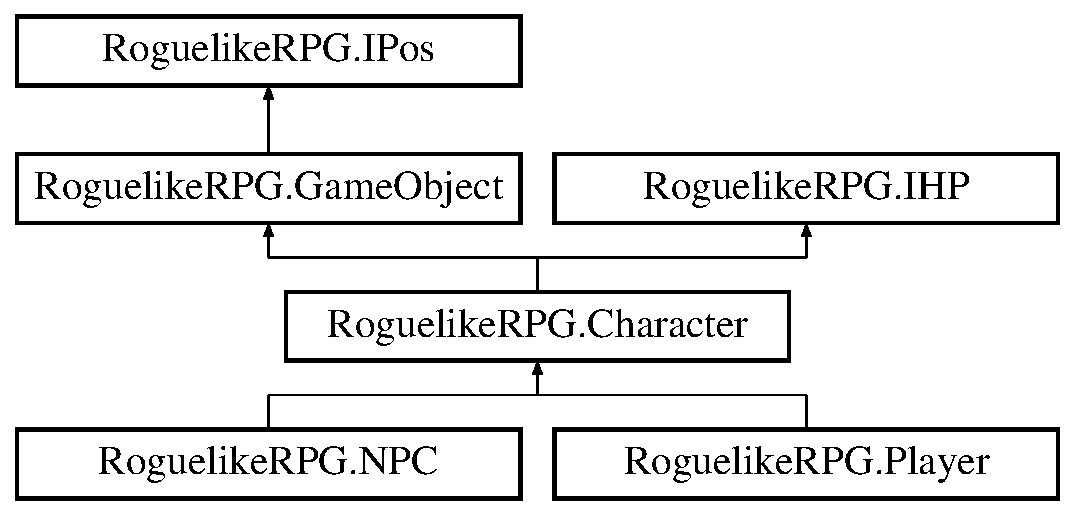
\includegraphics[height=4.000000cm]{class_roguelike_r_p_g_1_1_character}
\end{center}
\end{figure}
\subsection*{Public Member Functions}
\begin{DoxyCompactItemize}
\item 
virtual void \mbox{\hyperlink{class_roguelike_r_p_g_1_1_character_a9b78a6de5cabe2c59d0b965733d9d63b}{Move}} (char dir, \mbox{\hyperlink{class_roguelike_r_p_g_1_1_grid}{Grid}} grid)
\begin{DoxyCompactList}\small\item\em Changes the characters cordinates depending on the direction given. \end{DoxyCompactList}\end{DoxyCompactItemize}
\subsection*{Properties}
\begin{DoxyCompactItemize}
\item 
float \mbox{\hyperlink{class_roguelike_r_p_g_1_1_character_a9d6a6a907e8d26c967218e7cf5ea02c7}{HP}}\hspace{0.3cm}{\ttfamily  \mbox{[}get, set\mbox{]}}
\begin{DoxyCompactList}\small\item\em Holds health value. \end{DoxyCompactList}\end{DoxyCompactItemize}


\subsection{Detailed Description}
Class that handles all of the functions in regards to the \mbox{\hyperlink{class_roguelike_r_p_g_1_1_character}{Character}} sub type from \mbox{\hyperlink{class_roguelike_r_p_g_1_1_game_object}{Game\+Object}}. 



\subsection{Member Function Documentation}
\mbox{\Hypertarget{class_roguelike_r_p_g_1_1_character_a9b78a6de5cabe2c59d0b965733d9d63b}\label{class_roguelike_r_p_g_1_1_character_a9b78a6de5cabe2c59d0b965733d9d63b}} 
\index{Roguelike\+R\+P\+G\+::\+Character@{Roguelike\+R\+P\+G\+::\+Character}!Move@{Move}}
\index{Move@{Move}!Roguelike\+R\+P\+G\+::\+Character@{Roguelike\+R\+P\+G\+::\+Character}}
\subsubsection{\texorpdfstring{Move()}{Move()}}
{\footnotesize\ttfamily virtual void Roguelike\+R\+P\+G.\+Character.\+Move (\begin{DoxyParamCaption}\item[{char}]{dir,  }\item[{\mbox{\hyperlink{class_roguelike_r_p_g_1_1_grid}{Grid}}}]{grid }\end{DoxyParamCaption})\hspace{0.3cm}{\ttfamily [inline]}, {\ttfamily [virtual]}}



Changes the characters cordinates depending on the direction given. 


\begin{DoxyParams}{Parameters}
{\em dir} & \\
\hline
{\em grid} & \\
\hline
\end{DoxyParams}


\subsection{Property Documentation}
\mbox{\Hypertarget{class_roguelike_r_p_g_1_1_character_a9d6a6a907e8d26c967218e7cf5ea02c7}\label{class_roguelike_r_p_g_1_1_character_a9d6a6a907e8d26c967218e7cf5ea02c7}} 
\index{Roguelike\+R\+P\+G\+::\+Character@{Roguelike\+R\+P\+G\+::\+Character}!HP@{HP}}
\index{HP@{HP}!Roguelike\+R\+P\+G\+::\+Character@{Roguelike\+R\+P\+G\+::\+Character}}
\subsubsection{\texorpdfstring{HP}{HP}}
{\footnotesize\ttfamily float Roguelike\+R\+P\+G.\+Character.\+HP\hspace{0.3cm}{\ttfamily [get]}, {\ttfamily [set]}}



Holds health value. 



The documentation for this class was generated from the following file\+:\begin{DoxyCompactItemize}
\item 
Character.\+cs\end{DoxyCompactItemize}

\hypertarget{class_roguelike_r_p_g_1_1_food}{}\section{Roguelike\+R\+P\+G.\+Food Class Reference}
\label{class_roguelike_r_p_g_1_1_food}\index{Roguelike\+R\+P\+G.\+Food@{Roguelike\+R\+P\+G.\+Food}}


Class that handles all of the functions in regards to the \mbox{\hyperlink{class_roguelike_r_p_g_1_1_food}{Food}} sub type from items.  


Inheritance diagram for Roguelike\+R\+P\+G.\+Food\+:\begin{figure}[H]
\begin{center}
\leavevmode
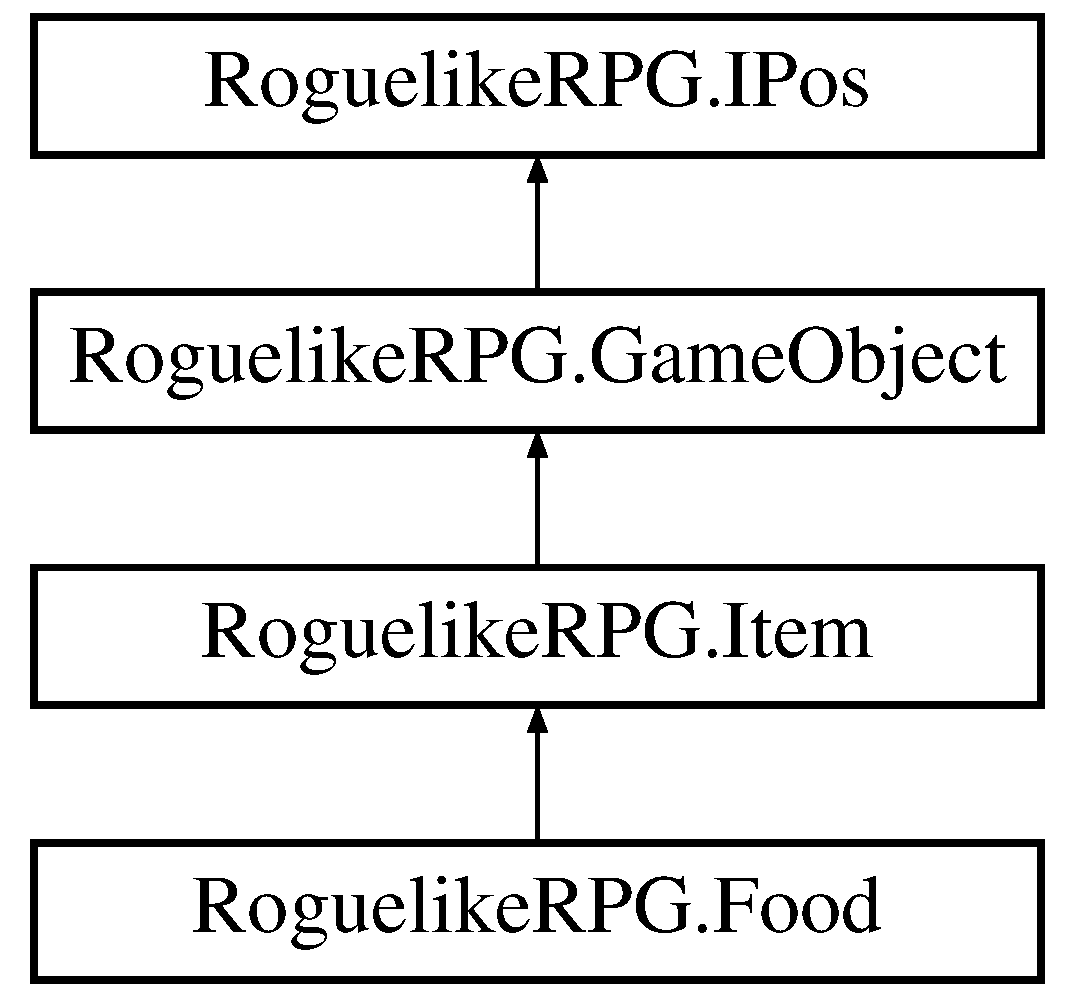
\includegraphics[height=4.000000cm]{class_roguelike_r_p_g_1_1_food}
\end{center}
\end{figure}
\subsection*{Public Member Functions}
\begin{DoxyCompactItemize}
\item 
\mbox{\hyperlink{class_roguelike_r_p_g_1_1_food_adab425fc62ac669c0c0155f1fa109dab}{Food}} (\mbox{\hyperlink{struct_roguelike_r_p_g_1_1_object_data}{Object\+Data}} obj, int x, int y)
\begin{DoxyCompactList}\small\item\em Initializer of the \mbox{\hyperlink{class_roguelike_r_p_g_1_1_food}{Food}} Object. \end{DoxyCompactList}\item 
void \mbox{\hyperlink{class_roguelike_r_p_g_1_1_food_a422486d8f892efec7859a7a62fa39af0}{Use}} (\mbox{\hyperlink{class_roguelike_r_p_g_1_1_player}{Player}} p)
\begin{DoxyCompactList}\small\item\em Uses the item, removing it from the backpack and adding the health it gives, while making sure there isnt an overheal. \end{DoxyCompactList}\end{DoxyCompactItemize}
\subsection*{Properties}
\begin{DoxyCompactItemize}
\item 
float \mbox{\hyperlink{class_roguelike_r_p_g_1_1_food_a644766aa45f4a118e3b2857c21221352}{H\+P\+Increase}}\hspace{0.3cm}{\ttfamily  \mbox{[}get, set\mbox{]}}
\begin{DoxyCompactList}\small\item\em Holds the ammount of HP said item will add when consumed. \end{DoxyCompactList}\end{DoxyCompactItemize}


\subsection{Detailed Description}
Class that handles all of the functions in regards to the \mbox{\hyperlink{class_roguelike_r_p_g_1_1_food}{Food}} sub type from items. 



\subsection{Constructor \& Destructor Documentation}
\mbox{\Hypertarget{class_roguelike_r_p_g_1_1_food_adab425fc62ac669c0c0155f1fa109dab}\label{class_roguelike_r_p_g_1_1_food_adab425fc62ac669c0c0155f1fa109dab}} 
\index{Roguelike\+R\+P\+G\+::\+Food@{Roguelike\+R\+P\+G\+::\+Food}!Food@{Food}}
\index{Food@{Food}!Roguelike\+R\+P\+G\+::\+Food@{Roguelike\+R\+P\+G\+::\+Food}}
\subsubsection{\texorpdfstring{Food()}{Food()}}
{\footnotesize\ttfamily Roguelike\+R\+P\+G.\+Food.\+Food (\begin{DoxyParamCaption}\item[{\mbox{\hyperlink{struct_roguelike_r_p_g_1_1_object_data}{Object\+Data}}}]{obj,  }\item[{int}]{x,  }\item[{int}]{y }\end{DoxyParamCaption})\hspace{0.3cm}{\ttfamily [inline]}}



Initializer of the \mbox{\hyperlink{class_roguelike_r_p_g_1_1_food}{Food}} Object. 


\begin{DoxyParams}{Parameters}
{\em obj} & Struct that is used to define the object.\\
\hline
{\em x} & X location\\
\hline
{\em y} & Y location\\
\hline
\end{DoxyParams}


\subsection{Member Function Documentation}
\mbox{\Hypertarget{class_roguelike_r_p_g_1_1_food_a422486d8f892efec7859a7a62fa39af0}\label{class_roguelike_r_p_g_1_1_food_a422486d8f892efec7859a7a62fa39af0}} 
\index{Roguelike\+R\+P\+G\+::\+Food@{Roguelike\+R\+P\+G\+::\+Food}!Use@{Use}}
\index{Use@{Use}!Roguelike\+R\+P\+G\+::\+Food@{Roguelike\+R\+P\+G\+::\+Food}}
\subsubsection{\texorpdfstring{Use()}{Use()}}
{\footnotesize\ttfamily void Roguelike\+R\+P\+G.\+Food.\+Use (\begin{DoxyParamCaption}\item[{\mbox{\hyperlink{class_roguelike_r_p_g_1_1_player}{Player}}}]{p }\end{DoxyParamCaption})\hspace{0.3cm}{\ttfamily [inline]}}



Uses the item, removing it from the backpack and adding the health it gives, while making sure there isnt an overheal. 


\begin{DoxyParams}{Parameters}
{\em p} & \\
\hline
\end{DoxyParams}


\subsection{Property Documentation}
\mbox{\Hypertarget{class_roguelike_r_p_g_1_1_food_a644766aa45f4a118e3b2857c21221352}\label{class_roguelike_r_p_g_1_1_food_a644766aa45f4a118e3b2857c21221352}} 
\index{Roguelike\+R\+P\+G\+::\+Food@{Roguelike\+R\+P\+G\+::\+Food}!H\+P\+Increase@{H\+P\+Increase}}
\index{H\+P\+Increase@{H\+P\+Increase}!Roguelike\+R\+P\+G\+::\+Food@{Roguelike\+R\+P\+G\+::\+Food}}
\subsubsection{\texorpdfstring{H\+P\+Increase}{HPIncrease}}
{\footnotesize\ttfamily float Roguelike\+R\+P\+G.\+Food.\+H\+P\+Increase\hspace{0.3cm}{\ttfamily [get]}, {\ttfamily [set]}}



Holds the ammount of HP said item will add when consumed. 



The documentation for this class was generated from the following file\+:\begin{DoxyCompactItemize}
\item 
Food.\+cs\end{DoxyCompactItemize}

\hypertarget{class_roguelike_r_p_g_1_1_game_loop}{}\section{Roguelike\+R\+P\+G.\+Game\+Loop Class Reference}
\label{class_roguelike_r_p_g_1_1_game_loop}\index{Roguelike\+R\+P\+G.\+Game\+Loop@{Roguelike\+R\+P\+G.\+Game\+Loop}}


Class that storages some important variables from the game itself, like the state and the lvl  


\subsection*{Public Member Functions}
\begin{DoxyCompactItemize}
\item 
void \mbox{\hyperlink{class_roguelike_r_p_g_1_1_game_loop_aa012d706ad4d98f0f6fb321d37638c3c}{Loop}} (\mbox{\hyperlink{class_roguelike_r_p_g_1_1_player}{Player}} player, \mbox{\hyperlink{class_roguelike_r_p_g_1_1_grid}{Grid}} grid)
\begin{DoxyCompactList}\small\item\em Function that seeks the win/lose conditions \end{DoxyCompactList}\end{DoxyCompactItemize}
\subsection*{Properties}
\begin{DoxyCompactItemize}
\item 
\mbox{\Hypertarget{class_roguelike_r_p_g_1_1_game_loop_aab86497d0428409f1d5b8412f8ac775a}\label{class_roguelike_r_p_g_1_1_game_loop_aab86497d0428409f1d5b8412f8ac775a}} 
string {\bfseries State}\hspace{0.3cm}{\ttfamily  \mbox{[}get, set\mbox{]}}
\item 
\mbox{\Hypertarget{class_roguelike_r_p_g_1_1_game_loop_a636d816b0a16620f1776cbdaeadb9f6b}\label{class_roguelike_r_p_g_1_1_game_loop_a636d816b0a16620f1776cbdaeadb9f6b}} 
int {\bfseries Level}\hspace{0.3cm}{\ttfamily  \mbox{[}get, set\mbox{]}}
\item 
\mbox{\Hypertarget{class_roguelike_r_p_g_1_1_game_loop_ad53ffbdbf9f9780b9ae78bef180806fd}\label{class_roguelike_r_p_g_1_1_game_loop_ad53ffbdbf9f9780b9ae78bef180806fd}} 
bool {\bfseries in\+Game}\hspace{0.3cm}{\ttfamily  \mbox{[}get, set\mbox{]}}
\end{DoxyCompactItemize}


\subsection{Detailed Description}
Class that storages some important variables from the game itself, like the state and the lvl 



\subsection{Member Function Documentation}
\mbox{\Hypertarget{class_roguelike_r_p_g_1_1_game_loop_aa012d706ad4d98f0f6fb321d37638c3c}\label{class_roguelike_r_p_g_1_1_game_loop_aa012d706ad4d98f0f6fb321d37638c3c}} 
\index{Roguelike\+R\+P\+G\+::\+Game\+Loop@{Roguelike\+R\+P\+G\+::\+Game\+Loop}!Loop@{Loop}}
\index{Loop@{Loop}!Roguelike\+R\+P\+G\+::\+Game\+Loop@{Roguelike\+R\+P\+G\+::\+Game\+Loop}}
\subsubsection{\texorpdfstring{Loop()}{Loop()}}
{\footnotesize\ttfamily void Roguelike\+R\+P\+G.\+Game\+Loop.\+Loop (\begin{DoxyParamCaption}\item[{\mbox{\hyperlink{class_roguelike_r_p_g_1_1_player}{Player}}}]{player,  }\item[{\mbox{\hyperlink{class_roguelike_r_p_g_1_1_grid}{Grid}}}]{grid }\end{DoxyParamCaption})\hspace{0.3cm}{\ttfamily [inline]}}



Function that seeks the win/lose conditions 


\begin{DoxyParams}{Parameters}
{\em player} & \\
\hline
{\em grid} & \\
\hline
\end{DoxyParams}


The documentation for this class was generated from the following file\+:\begin{DoxyCompactItemize}
\item 
Game\+Loop.\+cs\end{DoxyCompactItemize}

\hypertarget{class_roguelike_r_p_g_1_1_game_object}{}\section{Roguelike\+R\+P\+G.\+Game\+Object Class Reference}
\label{class_roguelike_r_p_g_1_1_game_object}\index{Roguelike\+R\+P\+G.\+Game\+Object@{Roguelike\+R\+P\+G.\+Game\+Object}}


Abstract class that holds information for the objects.  


Inheritance diagram for Roguelike\+R\+P\+G.\+Game\+Object\+:\begin{figure}[H]
\begin{center}
\leavevmode
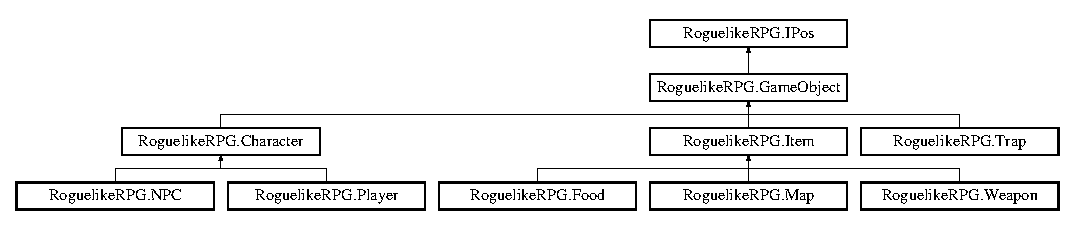
\includegraphics[height=2.589595cm]{class_roguelike_r_p_g_1_1_game_object}
\end{center}
\end{figure}
\subsection*{Properties}
\begin{DoxyCompactItemize}
\item 
\mbox{\Hypertarget{class_roguelike_r_p_g_1_1_game_object_ac74edfab8ad8acb0286337a78ae0c5ae}\label{class_roguelike_r_p_g_1_1_game_object_ac74edfab8ad8acb0286337a78ae0c5ae}} 
int {\bfseries ID}\hspace{0.3cm}{\ttfamily  \mbox{[}get, set\mbox{]}}
\item 
\mbox{\Hypertarget{class_roguelike_r_p_g_1_1_game_object_a10d65dd355cb9d8d2fe56a01894809ef}\label{class_roguelike_r_p_g_1_1_game_object_a10d65dd355cb9d8d2fe56a01894809ef}} 
string {\bfseries Name}\hspace{0.3cm}{\ttfamily  \mbox{[}get, set\mbox{]}}
\item 
\mbox{\Hypertarget{class_roguelike_r_p_g_1_1_game_object_a98f1d2ad9bc6ec7e7a71071aae35ba03}\label{class_roguelike_r_p_g_1_1_game_object_a98f1d2ad9bc6ec7e7a71071aae35ba03}} 
int {\bfseries X}\hspace{0.3cm}{\ttfamily  \mbox{[}get, set\mbox{]}}
\item 
\mbox{\Hypertarget{class_roguelike_r_p_g_1_1_game_object_a0c27f37c3a04fdb5203cbc3b46ddcc0a}\label{class_roguelike_r_p_g_1_1_game_object_a0c27f37c3a04fdb5203cbc3b46ddcc0a}} 
int {\bfseries Y}\hspace{0.3cm}{\ttfamily  \mbox{[}get, set\mbox{]}}
\item 
\mbox{\Hypertarget{class_roguelike_r_p_g_1_1_game_object_ab51d4d46d06a314e2d4c39ed57c29c9d}\label{class_roguelike_r_p_g_1_1_game_object_ab51d4d46d06a314e2d4c39ed57c29c9d}} 
string {\bfseries Icon}\hspace{0.3cm}{\ttfamily  \mbox{[}get, set\mbox{]}}
\item 
\mbox{\Hypertarget{class_roguelike_r_p_g_1_1_game_object_af9101b4a662b532e43b9d21f2594ddcd}\label{class_roguelike_r_p_g_1_1_game_object_af9101b4a662b532e43b9d21f2594ddcd}} 
int {\bfseries Pos\+In\+Tile}\hspace{0.3cm}{\ttfamily  \mbox{[}get, set\mbox{]}}
\end{DoxyCompactItemize}


\subsection{Detailed Description}
Abstract class that holds information for the objects. 



The documentation for this class was generated from the following file\+:\begin{DoxyCompactItemize}
\item 
Game\+Object.\+cs\end{DoxyCompactItemize}

\hypertarget{class_roguelike_r_p_g_1_1_grid}{}\section{Roguelike\+R\+P\+G.\+Grid Class Reference}
\label{class_roguelike_r_p_g_1_1_grid}\index{Roguelike\+R\+P\+G.\+Grid@{Roguelike\+R\+P\+G.\+Grid}}
\subsection*{Public Member Functions}
\begin{DoxyCompactItemize}
\item 
\mbox{\Hypertarget{class_roguelike_r_p_g_1_1_grid_a91be273f5c588230875e727f69956db9}\label{class_roguelike_r_p_g_1_1_grid_a91be273f5c588230875e727f69956db9}} 
void {\bfseries Update\+Positions} ()
\item 
\mbox{\Hypertarget{class_roguelike_r_p_g_1_1_grid_aa1811392b11d7f50de49a599128832fe}\label{class_roguelike_r_p_g_1_1_grid_aa1811392b11d7f50de49a599128832fe}} 
List$<$ \mbox{\hyperlink{class_roguelike_r_p_g_1_1_game_object}{Game\+Object}} $>$ {\bfseries Get\+Game\+Objects\+Of\+Type$<$ T $>$} ()
\item 
\mbox{\Hypertarget{class_roguelike_r_p_g_1_1_grid_a025f9368d08af8faf4d3e25765f60aaa}\label{class_roguelike_r_p_g_1_1_grid_a025f9368d08af8faf4d3e25765f60aaa}} 
void {\bfseries Update\+Known\+Places} (\mbox{\hyperlink{class_roguelike_r_p_g_1_1_player}{Player}} p)
\item 
\mbox{\Hypertarget{class_roguelike_r_p_g_1_1_grid_a9997a333c0f023d83b56ca14bd592deb}\label{class_roguelike_r_p_g_1_1_grid_a9997a333c0f023d83b56ca14bd592deb}} 
void {\bfseries Fill} (int level)
\end{DoxyCompactItemize}
\subsection*{Public Attributes}
\begin{DoxyCompactItemize}
\item 
\mbox{\Hypertarget{class_roguelike_r_p_g_1_1_grid_ae8f1fe9e449ba7110a910631969c4371}\label{class_roguelike_r_p_g_1_1_grid_ae8f1fe9e449ba7110a910631969c4371}} 
\mbox{\hyperlink{class_roguelike_r_p_g_1_1_tile}{Tile}} \mbox{[},\mbox{]} {\bfseries tiles} = new \mbox{\hyperlink{class_roguelike_r_p_g_1_1_tile}{Tile}}\mbox{[}8, 8\mbox{]}
\end{DoxyCompactItemize}


The documentation for this class was generated from the following file\+:\begin{DoxyCompactItemize}
\item 
Grid.\+cs\end{DoxyCompactItemize}

\hypertarget{interface_roguelike_r_p_g_1_1_i_attack_power}{}\section{Roguelike\+R\+P\+G.\+I\+Attack\+Power Interface Reference}
\label{interface_roguelike_r_p_g_1_1_i_attack_power}\index{Roguelike\+R\+P\+G.\+I\+Attack\+Power@{Roguelike\+R\+P\+G.\+I\+Attack\+Power}}


Interface that holds the Attack Power values.  


Inheritance diagram for Roguelike\+R\+P\+G.\+I\+Attack\+Power\+:\begin{figure}[H]
\begin{center}
\leavevmode
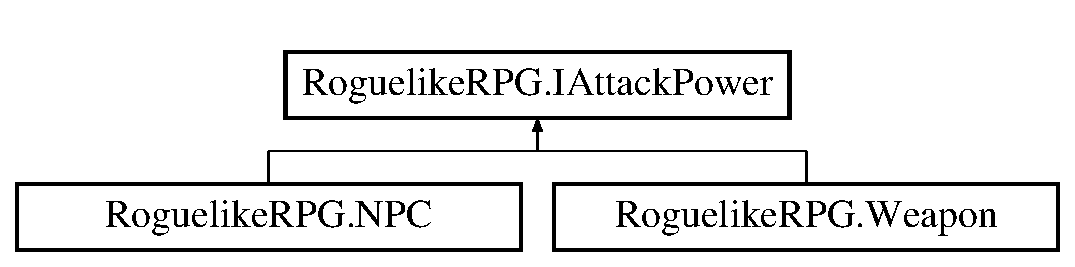
\includegraphics[height=2.000000cm]{interface_roguelike_r_p_g_1_1_i_attack_power}
\end{center}
\end{figure}
\subsection*{Properties}
\begin{DoxyCompactItemize}
\item 
\mbox{\Hypertarget{interface_roguelike_r_p_g_1_1_i_attack_power_a42a0c319db9e218045c4fd2b57d6e582}\label{interface_roguelike_r_p_g_1_1_i_attack_power_a42a0c319db9e218045c4fd2b57d6e582}} 
float {\bfseries Attack\+Power}\hspace{0.3cm}{\ttfamily  \mbox{[}get, set\mbox{]}}
\end{DoxyCompactItemize}


\subsection{Detailed Description}
Interface that holds the Attack Power values. 



The documentation for this interface was generated from the following file\+:\begin{DoxyCompactItemize}
\item 
I\+Attack\+Power.\+cs\end{DoxyCompactItemize}

\hypertarget{interface_roguelike_r_p_g_1_1_i_h_p}{}\section{Roguelike\+R\+P\+G.\+I\+HP Interface Reference}
\label{interface_roguelike_r_p_g_1_1_i_h_p}\index{Roguelike\+R\+P\+G.\+I\+HP@{Roguelike\+R\+P\+G.\+I\+HP}}


Interface that holds the health values.  


Inheritance diagram for Roguelike\+R\+P\+G.\+I\+HP\+:\begin{figure}[H]
\begin{center}
\leavevmode
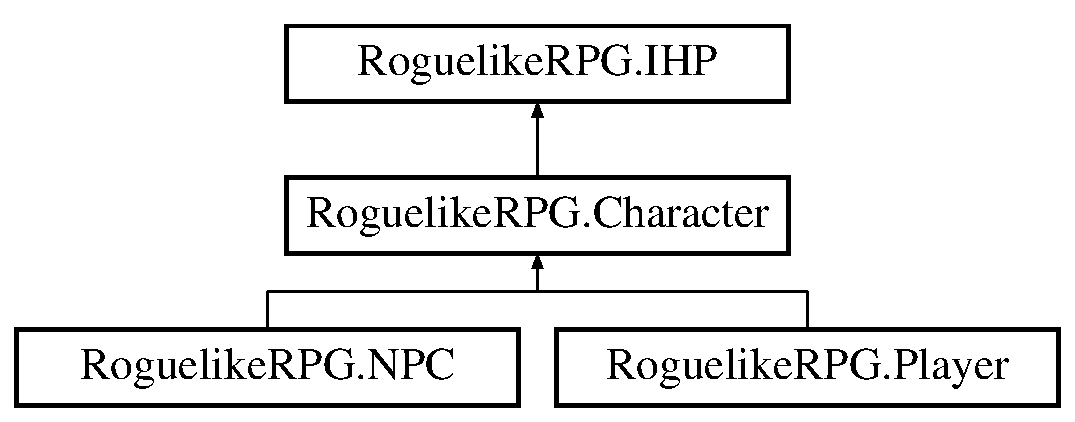
\includegraphics[height=3.000000cm]{interface_roguelike_r_p_g_1_1_i_h_p}
\end{center}
\end{figure}
\subsection*{Properties}
\begin{DoxyCompactItemize}
\item 
\mbox{\Hypertarget{interface_roguelike_r_p_g_1_1_i_h_p_a4f0ed9c0d4a526d5eee62b2371e80408}\label{interface_roguelike_r_p_g_1_1_i_h_p_a4f0ed9c0d4a526d5eee62b2371e80408}} 
float {\bfseries HP}\hspace{0.3cm}{\ttfamily  \mbox{[}get, set\mbox{]}}
\end{DoxyCompactItemize}


\subsection{Detailed Description}
Interface that holds the health values. 



The documentation for this interface was generated from the following file\+:\begin{DoxyCompactItemize}
\item 
I\+H\+P.\+cs\end{DoxyCompactItemize}

\hypertarget{class_roguelike_r_p_g_1_1_input_manager}{}\section{Roguelike\+R\+P\+G.\+Input\+Manager Class Reference}
\label{class_roguelike_r_p_g_1_1_input_manager}\index{Roguelike\+R\+P\+G.\+Input\+Manager@{Roguelike\+R\+P\+G.\+Input\+Manager}}


 


\subsection*{Public Member Functions}
\begin{DoxyCompactItemize}
\item 
\mbox{\hyperlink{class_roguelike_r_p_g_1_1_input_manager_a638a30fe668a76236a2465c759941e1f}{Input\+Manager}} (\mbox{\hyperlink{class_roguelike_r_p_g_1_1_player}{Player}} player, \mbox{\hyperlink{class_roguelike_r_p_g_1_1_grid}{Grid}} grid, \mbox{\hyperlink{class_roguelike_r_p_g_1_1_renderer}{Renderer}} render, \mbox{\hyperlink{class_roguelike_r_p_g_1_1_game_loop}{Game\+Loop}} game\+Loop, \mbox{\hyperlink{class_roguelike_r_p_g_1_1_map}{Map}} map)
\begin{DoxyCompactList}\small\item\em Class constructor \end{DoxyCompactList}\item 
void \mbox{\hyperlink{class_roguelike_r_p_g_1_1_input_manager_a4cf1240d67c0b5f014eb44a752bd973e}{Turn\+Command}} ()
\begin{DoxyCompactList}\small\item\em Function that catches the input for the actual turn \end{DoxyCompactList}\item 
void \mbox{\hyperlink{class_roguelike_r_p_g_1_1_input_manager_aec0961d74c0742a206f3e0af0cafd2f7}{Start\+Screen\+Command}} ()
\begin{DoxyCompactList}\small\item\em Function that catches the inputs from the Start Screen \end{DoxyCompactList}\item 
void \mbox{\hyperlink{class_roguelike_r_p_g_1_1_input_manager_a320b37790da7ab766eb987471c893a2a}{Credit\+Commands}} ()
\begin{DoxyCompactList}\small\item\em Function that reads the commands from the Credit Screen \end{DoxyCompactList}\end{DoxyCompactItemize}


\subsection{Detailed Description}


Class that deals with the inputs from the player 

\subsection{Constructor \& Destructor Documentation}
\mbox{\Hypertarget{class_roguelike_r_p_g_1_1_input_manager_a638a30fe668a76236a2465c759941e1f}\label{class_roguelike_r_p_g_1_1_input_manager_a638a30fe668a76236a2465c759941e1f}} 
\index{Roguelike\+R\+P\+G\+::\+Input\+Manager@{Roguelike\+R\+P\+G\+::\+Input\+Manager}!Input\+Manager@{Input\+Manager}}
\index{Input\+Manager@{Input\+Manager}!Roguelike\+R\+P\+G\+::\+Input\+Manager@{Roguelike\+R\+P\+G\+::\+Input\+Manager}}
\subsubsection{\texorpdfstring{Input\+Manager()}{InputManager()}}
{\footnotesize\ttfamily Roguelike\+R\+P\+G.\+Input\+Manager.\+Input\+Manager (\begin{DoxyParamCaption}\item[{\mbox{\hyperlink{class_roguelike_r_p_g_1_1_player}{Player}}}]{player,  }\item[{\mbox{\hyperlink{class_roguelike_r_p_g_1_1_grid}{Grid}}}]{grid,  }\item[{\mbox{\hyperlink{class_roguelike_r_p_g_1_1_renderer}{Renderer}}}]{render,  }\item[{\mbox{\hyperlink{class_roguelike_r_p_g_1_1_game_loop}{Game\+Loop}}}]{game\+Loop,  }\item[{\mbox{\hyperlink{class_roguelike_r_p_g_1_1_map}{Map}}}]{map }\end{DoxyParamCaption})\hspace{0.3cm}{\ttfamily [inline]}}



Class constructor 


\begin{DoxyParams}{Parameters}
{\em player} & \\
\hline
{\em grid} & \\
\hline
{\em render} & \\
\hline
{\em game\+Loop} & \\
\hline
{\em map} & \\
\hline
\end{DoxyParams}


\subsection{Member Function Documentation}
\mbox{\Hypertarget{class_roguelike_r_p_g_1_1_input_manager_a320b37790da7ab766eb987471c893a2a}\label{class_roguelike_r_p_g_1_1_input_manager_a320b37790da7ab766eb987471c893a2a}} 
\index{Roguelike\+R\+P\+G\+::\+Input\+Manager@{Roguelike\+R\+P\+G\+::\+Input\+Manager}!Credit\+Commands@{Credit\+Commands}}
\index{Credit\+Commands@{Credit\+Commands}!Roguelike\+R\+P\+G\+::\+Input\+Manager@{Roguelike\+R\+P\+G\+::\+Input\+Manager}}
\subsubsection{\texorpdfstring{Credit\+Commands()}{CreditCommands()}}
{\footnotesize\ttfamily void Roguelike\+R\+P\+G.\+Input\+Manager.\+Credit\+Commands (\begin{DoxyParamCaption}{ }\end{DoxyParamCaption})\hspace{0.3cm}{\ttfamily [inline]}}



Function that reads the commands from the Credit Screen 

\mbox{\Hypertarget{class_roguelike_r_p_g_1_1_input_manager_aec0961d74c0742a206f3e0af0cafd2f7}\label{class_roguelike_r_p_g_1_1_input_manager_aec0961d74c0742a206f3e0af0cafd2f7}} 
\index{Roguelike\+R\+P\+G\+::\+Input\+Manager@{Roguelike\+R\+P\+G\+::\+Input\+Manager}!Start\+Screen\+Command@{Start\+Screen\+Command}}
\index{Start\+Screen\+Command@{Start\+Screen\+Command}!Roguelike\+R\+P\+G\+::\+Input\+Manager@{Roguelike\+R\+P\+G\+::\+Input\+Manager}}
\subsubsection{\texorpdfstring{Start\+Screen\+Command()}{StartScreenCommand()}}
{\footnotesize\ttfamily void Roguelike\+R\+P\+G.\+Input\+Manager.\+Start\+Screen\+Command (\begin{DoxyParamCaption}{ }\end{DoxyParamCaption})\hspace{0.3cm}{\ttfamily [inline]}}



Function that catches the inputs from the Start Screen 

\mbox{\Hypertarget{class_roguelike_r_p_g_1_1_input_manager_a4cf1240d67c0b5f014eb44a752bd973e}\label{class_roguelike_r_p_g_1_1_input_manager_a4cf1240d67c0b5f014eb44a752bd973e}} 
\index{Roguelike\+R\+P\+G\+::\+Input\+Manager@{Roguelike\+R\+P\+G\+::\+Input\+Manager}!Turn\+Command@{Turn\+Command}}
\index{Turn\+Command@{Turn\+Command}!Roguelike\+R\+P\+G\+::\+Input\+Manager@{Roguelike\+R\+P\+G\+::\+Input\+Manager}}
\subsubsection{\texorpdfstring{Turn\+Command()}{TurnCommand()}}
{\footnotesize\ttfamily void Roguelike\+R\+P\+G.\+Input\+Manager.\+Turn\+Command (\begin{DoxyParamCaption}{ }\end{DoxyParamCaption})\hspace{0.3cm}{\ttfamily [inline]}}



Function that catches the input for the actual turn 



The documentation for this class was generated from the following file\+:\begin{DoxyCompactItemize}
\item 
Input\+Manager.\+cs\end{DoxyCompactItemize}

\hypertarget{interface_roguelike_r_p_g_1_1_i_pos}{}\section{Roguelike\+R\+P\+G.\+I\+Pos Interface Reference}
\label{interface_roguelike_r_p_g_1_1_i_pos}\index{Roguelike\+R\+P\+G.\+I\+Pos@{Roguelike\+R\+P\+G.\+I\+Pos}}


Interface that holds the positional values.  


Inheritance diagram for Roguelike\+R\+P\+G.\+I\+Pos\+:\begin{figure}[H]
\begin{center}
\leavevmode
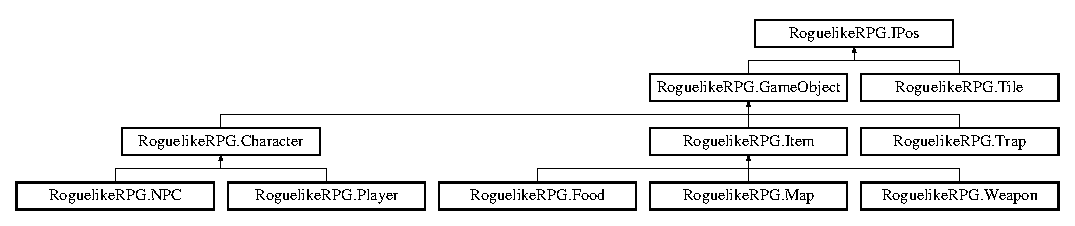
\includegraphics[height=2.589595cm]{interface_roguelike_r_p_g_1_1_i_pos}
\end{center}
\end{figure}
\subsection*{Properties}
\begin{DoxyCompactItemize}
\item 
\mbox{\Hypertarget{interface_roguelike_r_p_g_1_1_i_pos_aa40fce67404021056f1aef51a1e97e05}\label{interface_roguelike_r_p_g_1_1_i_pos_aa40fce67404021056f1aef51a1e97e05}} 
int {\bfseries X}\hspace{0.3cm}{\ttfamily  \mbox{[}get, set\mbox{]}}
\item 
\mbox{\Hypertarget{interface_roguelike_r_p_g_1_1_i_pos_afe7826d4293121d8f12f65ea6797563a}\label{interface_roguelike_r_p_g_1_1_i_pos_afe7826d4293121d8f12f65ea6797563a}} 
int {\bfseries Y}\hspace{0.3cm}{\ttfamily  \mbox{[}get, set\mbox{]}}
\end{DoxyCompactItemize}


\subsection{Detailed Description}
Interface that holds the positional values. 



The documentation for this interface was generated from the following file\+:\begin{DoxyCompactItemize}
\item 
I\+Pos.\+cs\end{DoxyCompactItemize}

\hypertarget{class_roguelike_r_p_g_1_1_item}{}\section{Roguelike\+R\+P\+G.\+Item Class Reference}
\label{class_roguelike_r_p_g_1_1_item}\index{Roguelike\+R\+P\+G.\+Item@{Roguelike\+R\+P\+G.\+Item}}


Abstract class that handles all of the functions in regards to the \mbox{\hyperlink{class_roguelike_r_p_g_1_1_item}{Item}} sub type from \mbox{\hyperlink{class_roguelike_r_p_g_1_1_game_object}{Game\+Object}}.  


Inheritance diagram for Roguelike\+R\+P\+G.\+Item\+:\begin{figure}[H]
\begin{center}
\leavevmode
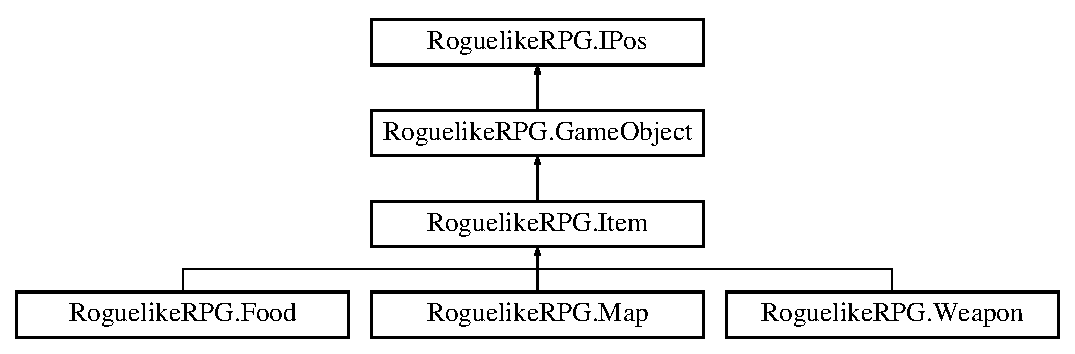
\includegraphics[height=4.000000cm]{class_roguelike_r_p_g_1_1_item}
\end{center}
\end{figure}
\subsection*{Public Member Functions}
\begin{DoxyCompactItemize}
\item 
virtual void \mbox{\hyperlink{class_roguelike_r_p_g_1_1_item_accf1844a3b2b53b75d8974ba14509c82}{Pick\+Up}} (\mbox{\hyperlink{class_roguelike_r_p_g_1_1_player}{Player}} p)
\begin{DoxyCompactList}\small\item\em Method to add specified item, to the specified player\textquotesingle{}s Backpack. \end{DoxyCompactList}\item 
virtual void \mbox{\hyperlink{class_roguelike_r_p_g_1_1_item_ae46e19cf36347b93f56704516c0c6618}{Drop}} ()
\begin{DoxyCompactList}\small\item\em Method to drop specified item, from the specified player\textquotesingle{}s Backpack. \end{DoxyCompactList}\end{DoxyCompactItemize}
\subsection*{Properties}
\begin{DoxyCompactItemize}
\item 
float \mbox{\hyperlink{class_roguelike_r_p_g_1_1_item_a3b805eda54cfe72ae368244ab07dda75}{Weight}}\hspace{0.3cm}{\ttfamily  \mbox{[}get, set\mbox{]}}
\begin{DoxyCompactList}\small\item\em Holds the Weight of said item. \end{DoxyCompactList}\end{DoxyCompactItemize}


\subsection{Detailed Description}
Abstract class that handles all of the functions in regards to the \mbox{\hyperlink{class_roguelike_r_p_g_1_1_item}{Item}} sub type from \mbox{\hyperlink{class_roguelike_r_p_g_1_1_game_object}{Game\+Object}}. 



\subsection{Member Function Documentation}
\mbox{\Hypertarget{class_roguelike_r_p_g_1_1_item_ae46e19cf36347b93f56704516c0c6618}\label{class_roguelike_r_p_g_1_1_item_ae46e19cf36347b93f56704516c0c6618}} 
\index{Roguelike\+R\+P\+G\+::\+Item@{Roguelike\+R\+P\+G\+::\+Item}!Drop@{Drop}}
\index{Drop@{Drop}!Roguelike\+R\+P\+G\+::\+Item@{Roguelike\+R\+P\+G\+::\+Item}}
\subsubsection{\texorpdfstring{Drop()}{Drop()}}
{\footnotesize\ttfamily virtual void Roguelike\+R\+P\+G.\+Item.\+Drop (\begin{DoxyParamCaption}{ }\end{DoxyParamCaption})\hspace{0.3cm}{\ttfamily [inline]}, {\ttfamily [virtual]}}



Method to drop specified item, from the specified player\textquotesingle{}s Backpack. 

\mbox{\Hypertarget{class_roguelike_r_p_g_1_1_item_accf1844a3b2b53b75d8974ba14509c82}\label{class_roguelike_r_p_g_1_1_item_accf1844a3b2b53b75d8974ba14509c82}} 
\index{Roguelike\+R\+P\+G\+::\+Item@{Roguelike\+R\+P\+G\+::\+Item}!Pick\+Up@{Pick\+Up}}
\index{Pick\+Up@{Pick\+Up}!Roguelike\+R\+P\+G\+::\+Item@{Roguelike\+R\+P\+G\+::\+Item}}
\subsubsection{\texorpdfstring{Pick\+Up()}{PickUp()}}
{\footnotesize\ttfamily virtual void Roguelike\+R\+P\+G.\+Item.\+Pick\+Up (\begin{DoxyParamCaption}\item[{\mbox{\hyperlink{class_roguelike_r_p_g_1_1_player}{Player}}}]{p }\end{DoxyParamCaption})\hspace{0.3cm}{\ttfamily [inline]}, {\ttfamily [virtual]}}



Method to add specified item, to the specified player\textquotesingle{}s Backpack. 


\begin{DoxyParams}{Parameters}
{\em p} & \\
\hline
\end{DoxyParams}


\subsection{Property Documentation}
\mbox{\Hypertarget{class_roguelike_r_p_g_1_1_item_a3b805eda54cfe72ae368244ab07dda75}\label{class_roguelike_r_p_g_1_1_item_a3b805eda54cfe72ae368244ab07dda75}} 
\index{Roguelike\+R\+P\+G\+::\+Item@{Roguelike\+R\+P\+G\+::\+Item}!Weight@{Weight}}
\index{Weight@{Weight}!Roguelike\+R\+P\+G\+::\+Item@{Roguelike\+R\+P\+G\+::\+Item}}
\subsubsection{\texorpdfstring{Weight}{Weight}}
{\footnotesize\ttfamily float Roguelike\+R\+P\+G.\+Item.\+Weight\hspace{0.3cm}{\ttfamily [get]}, {\ttfamily [set]}}



Holds the Weight of said item. 



The documentation for this class was generated from the following file\+:\begin{DoxyCompactItemize}
\item 
Item.\+cs\end{DoxyCompactItemize}

\hypertarget{class_roguelike_r_p_g_1_1_map}{}\section{Roguelike\+R\+P\+G.\+Map Class Reference}
\label{class_roguelike_r_p_g_1_1_map}\index{Roguelike\+R\+P\+G.\+Map@{Roguelike\+R\+P\+G.\+Map}}


Class that handles all of the functions in regards to the \mbox{\hyperlink{class_roguelike_r_p_g_1_1_map}{Map}} sub type from \mbox{\hyperlink{class_roguelike_r_p_g_1_1_item}{Item}}.  


Inheritance diagram for Roguelike\+R\+P\+G.\+Map\+:\begin{figure}[H]
\begin{center}
\leavevmode
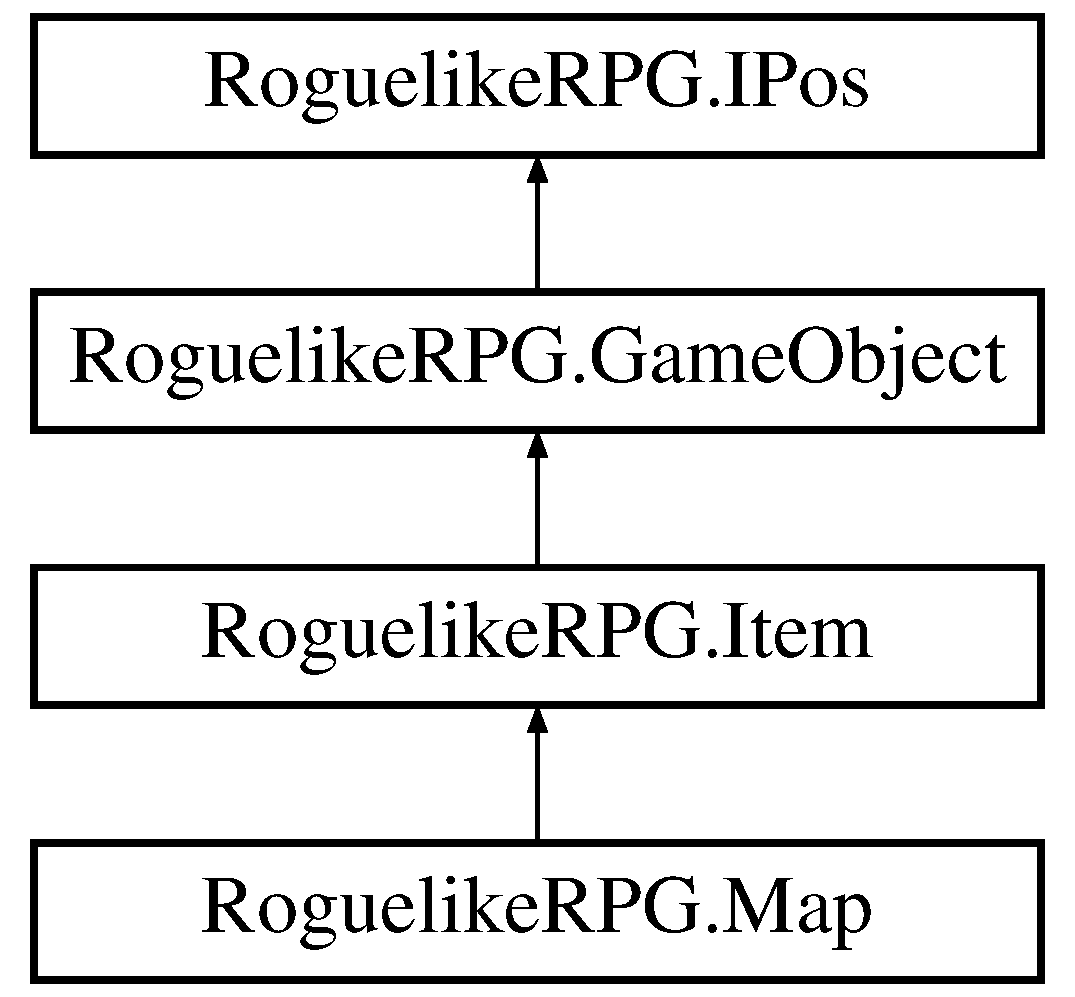
\includegraphics[height=4.000000cm]{class_roguelike_r_p_g_1_1_map}
\end{center}
\end{figure}
\subsection*{Public Member Functions}
\begin{DoxyCompactItemize}
\item 
\mbox{\hyperlink{class_roguelike_r_p_g_1_1_map_abaf4fc0e21d2f056464fb0e35d9cb14c}{Map}} (\mbox{\hyperlink{struct_roguelike_r_p_g_1_1_object_data}{Object\+Data}} obj, int x, int y)
\begin{DoxyCompactList}\small\item\em Manages the \mbox{\hyperlink{class_roguelike_r_p_g_1_1_map}{Map}} initialization. \end{DoxyCompactList}\item 
void \mbox{\hyperlink{class_roguelike_r_p_g_1_1_map_a7960c9dc9313df6cf3088578d17a07fa}{Use}} (\mbox{\hyperlink{class_roguelike_r_p_g_1_1_grid}{Grid}} grid)
\begin{DoxyCompactList}\small\item\em Manages the Use of the map. \end{DoxyCompactList}\end{DoxyCompactItemize}
\subsection*{Additional Inherited Members}


\subsection{Detailed Description}
Class that handles all of the functions in regards to the \mbox{\hyperlink{class_roguelike_r_p_g_1_1_map}{Map}} sub type from \mbox{\hyperlink{class_roguelike_r_p_g_1_1_item}{Item}}. 



\subsection{Constructor \& Destructor Documentation}
\mbox{\Hypertarget{class_roguelike_r_p_g_1_1_map_abaf4fc0e21d2f056464fb0e35d9cb14c}\label{class_roguelike_r_p_g_1_1_map_abaf4fc0e21d2f056464fb0e35d9cb14c}} 
\index{Roguelike\+R\+P\+G\+::\+Map@{Roguelike\+R\+P\+G\+::\+Map}!Map@{Map}}
\index{Map@{Map}!Roguelike\+R\+P\+G\+::\+Map@{Roguelike\+R\+P\+G\+::\+Map}}
\subsubsection{\texorpdfstring{Map()}{Map()}}
{\footnotesize\ttfamily Roguelike\+R\+P\+G.\+Map.\+Map (\begin{DoxyParamCaption}\item[{\mbox{\hyperlink{struct_roguelike_r_p_g_1_1_object_data}{Object\+Data}}}]{obj,  }\item[{int}]{x,  }\item[{int}]{y }\end{DoxyParamCaption})\hspace{0.3cm}{\ttfamily [inline]}}



Manages the \mbox{\hyperlink{class_roguelike_r_p_g_1_1_map}{Map}} initialization. 


\begin{DoxyParams}{Parameters}
{\em obj} & Struct holding the info of the map\\
\hline
{\em x} & X cordinate\\
\hline
{\em y} & Y cordinate\\
\hline
\end{DoxyParams}


\subsection{Member Function Documentation}
\mbox{\Hypertarget{class_roguelike_r_p_g_1_1_map_a7960c9dc9313df6cf3088578d17a07fa}\label{class_roguelike_r_p_g_1_1_map_a7960c9dc9313df6cf3088578d17a07fa}} 
\index{Roguelike\+R\+P\+G\+::\+Map@{Roguelike\+R\+P\+G\+::\+Map}!Use@{Use}}
\index{Use@{Use}!Roguelike\+R\+P\+G\+::\+Map@{Roguelike\+R\+P\+G\+::\+Map}}
\subsubsection{\texorpdfstring{Use()}{Use()}}
{\footnotesize\ttfamily void Roguelike\+R\+P\+G.\+Map.\+Use (\begin{DoxyParamCaption}\item[{\mbox{\hyperlink{class_roguelike_r_p_g_1_1_grid}{Grid}}}]{grid }\end{DoxyParamCaption})\hspace{0.3cm}{\ttfamily [inline]}}



Manages the Use of the map. 


\begin{DoxyParams}{Parameters}
{\em grid} & \\
\hline
\end{DoxyParams}


The documentation for this class was generated from the following file\+:\begin{DoxyCompactItemize}
\item 
Map.\+cs\end{DoxyCompactItemize}

\hypertarget{class_roguelike_r_p_g_1_1_n_p_c}{}\section{Roguelike\+R\+P\+G.\+N\+PC Class Reference}
\label{class_roguelike_r_p_g_1_1_n_p_c}\index{Roguelike\+R\+P\+G.\+N\+PC@{Roguelike\+R\+P\+G.\+N\+PC}}


Class that handles all of the functions in regards to the \mbox{\hyperlink{class_roguelike_r_p_g_1_1_n_p_c}{N\+PC}} sub type from \mbox{\hyperlink{class_roguelike_r_p_g_1_1_character}{Character}}.  


Inheritance diagram for Roguelike\+R\+P\+G.\+N\+PC\+:\begin{figure}[H]
\begin{center}
\leavevmode
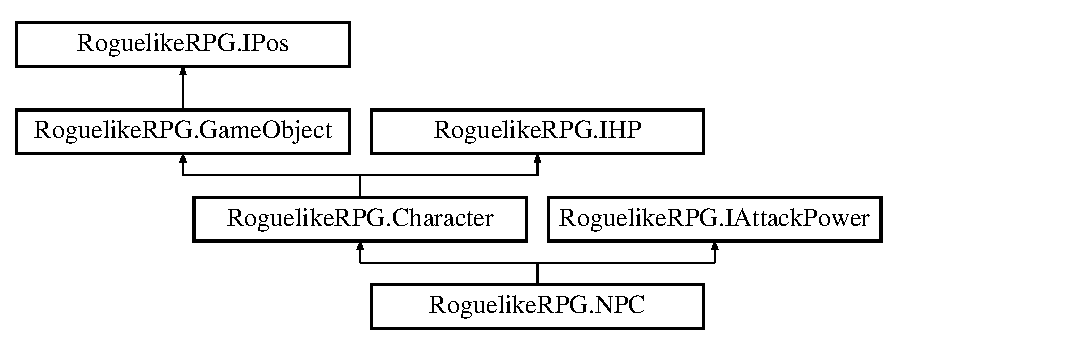
\includegraphics[height=4.000000cm]{class_roguelike_r_p_g_1_1_n_p_c}
\end{center}
\end{figure}
\subsection*{Public Member Functions}
\begin{DoxyCompactItemize}
\item 
\mbox{\hyperlink{class_roguelike_r_p_g_1_1_n_p_c_a2df0707bbdfb1078c414b87a1dd4cf5c}{N\+PC}} (\mbox{\hyperlink{struct_roguelike_r_p_g_1_1_object_data}{Object\+Data}} obj, int x, int y)
\begin{DoxyCompactList}\small\item\em Initializer of the \mbox{\hyperlink{class_roguelike_r_p_g_1_1_n_p_c}{N\+PC}} object on specified cordinates and the specified \mbox{\hyperlink{class_roguelike_r_p_g_1_1_n_p_c}{N\+PC}} characteristics. \end{DoxyCompactList}\end{DoxyCompactItemize}
\subsection*{Properties}
\begin{DoxyCompactItemize}
\item 
bool \mbox{\hyperlink{class_roguelike_r_p_g_1_1_n_p_c_a0573eb51eeafa976f5f4366ea1b14892}{Hostile}}\hspace{0.3cm}{\ttfamily  \mbox{[}get, set\mbox{]}}
\begin{DoxyCompactList}\small\item\em Handles the state of the \mbox{\hyperlink{class_roguelike_r_p_g_1_1_n_p_c}{N\+PC}}. \end{DoxyCompactList}\item 
float \mbox{\hyperlink{class_roguelike_r_p_g_1_1_n_p_c_a9cac8d5f5a1450aa17ff7739c109e7b8}{Attack\+Power}}\hspace{0.3cm}{\ttfamily  \mbox{[}get, set\mbox{]}}
\begin{DoxyCompactList}\small\item\em Handles the Attack\+Power of the \mbox{\hyperlink{class_roguelike_r_p_g_1_1_n_p_c}{N\+PC}}. \end{DoxyCompactList}\end{DoxyCompactItemize}


\subsection{Detailed Description}
Class that handles all of the functions in regards to the \mbox{\hyperlink{class_roguelike_r_p_g_1_1_n_p_c}{N\+PC}} sub type from \mbox{\hyperlink{class_roguelike_r_p_g_1_1_character}{Character}}. 



\subsection{Constructor \& Destructor Documentation}
\mbox{\Hypertarget{class_roguelike_r_p_g_1_1_n_p_c_a2df0707bbdfb1078c414b87a1dd4cf5c}\label{class_roguelike_r_p_g_1_1_n_p_c_a2df0707bbdfb1078c414b87a1dd4cf5c}} 
\index{Roguelike\+R\+P\+G\+::\+N\+PC@{Roguelike\+R\+P\+G\+::\+N\+PC}!N\+PC@{N\+PC}}
\index{N\+PC@{N\+PC}!Roguelike\+R\+P\+G\+::\+N\+PC@{Roguelike\+R\+P\+G\+::\+N\+PC}}
\subsubsection{\texorpdfstring{N\+P\+C()}{NPC()}}
{\footnotesize\ttfamily Roguelike\+R\+P\+G.\+N\+P\+C.\+N\+PC (\begin{DoxyParamCaption}\item[{\mbox{\hyperlink{struct_roguelike_r_p_g_1_1_object_data}{Object\+Data}}}]{obj,  }\item[{int}]{x,  }\item[{int}]{y }\end{DoxyParamCaption})\hspace{0.3cm}{\ttfamily [inline]}}



Initializer of the \mbox{\hyperlink{class_roguelike_r_p_g_1_1_n_p_c}{N\+PC}} object on specified cordinates and the specified \mbox{\hyperlink{class_roguelike_r_p_g_1_1_n_p_c}{N\+PC}} characteristics. 


\begin{DoxyParams}{Parameters}
{\em obj} & Struct that holds all of the \mbox{\hyperlink{class_roguelike_r_p_g_1_1_n_p_c}{N\+PC}} info\\
\hline
{\em x} & X cordinate\\
\hline
{\em y} & Y cordinate\\
\hline
\end{DoxyParams}


\subsection{Property Documentation}
\mbox{\Hypertarget{class_roguelike_r_p_g_1_1_n_p_c_a9cac8d5f5a1450aa17ff7739c109e7b8}\label{class_roguelike_r_p_g_1_1_n_p_c_a9cac8d5f5a1450aa17ff7739c109e7b8}} 
\index{Roguelike\+R\+P\+G\+::\+N\+PC@{Roguelike\+R\+P\+G\+::\+N\+PC}!Attack\+Power@{Attack\+Power}}
\index{Attack\+Power@{Attack\+Power}!Roguelike\+R\+P\+G\+::\+N\+PC@{Roguelike\+R\+P\+G\+::\+N\+PC}}
\subsubsection{\texorpdfstring{Attack\+Power}{AttackPower}}
{\footnotesize\ttfamily float Roguelike\+R\+P\+G.\+N\+P\+C.\+Attack\+Power\hspace{0.3cm}{\ttfamily [get]}, {\ttfamily [set]}}



Handles the Attack\+Power of the \mbox{\hyperlink{class_roguelike_r_p_g_1_1_n_p_c}{N\+PC}}. 

\mbox{\Hypertarget{class_roguelike_r_p_g_1_1_n_p_c_a0573eb51eeafa976f5f4366ea1b14892}\label{class_roguelike_r_p_g_1_1_n_p_c_a0573eb51eeafa976f5f4366ea1b14892}} 
\index{Roguelike\+R\+P\+G\+::\+N\+PC@{Roguelike\+R\+P\+G\+::\+N\+PC}!Hostile@{Hostile}}
\index{Hostile@{Hostile}!Roguelike\+R\+P\+G\+::\+N\+PC@{Roguelike\+R\+P\+G\+::\+N\+PC}}
\subsubsection{\texorpdfstring{Hostile}{Hostile}}
{\footnotesize\ttfamily bool Roguelike\+R\+P\+G.\+N\+P\+C.\+Hostile\hspace{0.3cm}{\ttfamily [get]}, {\ttfamily [set]}}



Handles the state of the \mbox{\hyperlink{class_roguelike_r_p_g_1_1_n_p_c}{N\+PC}}. 



The documentation for this class was generated from the following file\+:\begin{DoxyCompactItemize}
\item 
N\+P\+C.\+cs\end{DoxyCompactItemize}

\hypertarget{struct_roguelike_r_p_g_1_1_object_data}{}\section{Roguelike\+R\+P\+G.\+Object\+Data Struct Reference}
\label{struct_roguelike_r_p_g_1_1_object_data}\index{Roguelike\+R\+P\+G.\+Object\+Data@{Roguelike\+R\+P\+G.\+Object\+Data}}
\subsection*{Public Attributes}
\begin{DoxyCompactItemize}
\item 
\mbox{\Hypertarget{struct_roguelike_r_p_g_1_1_object_data_a9d04d55852c281b5c486605fd981b89c}\label{struct_roguelike_r_p_g_1_1_object_data_a9d04d55852c281b5c486605fd981b89c}} 
string {\bfseries name}
\item 
\mbox{\Hypertarget{struct_roguelike_r_p_g_1_1_object_data_a91977c7e1440f1b45cbf21157c6bf592}\label{struct_roguelike_r_p_g_1_1_object_data_a91977c7e1440f1b45cbf21157c6bf592}} 
string {\bfseries icon}
\item 
\mbox{\Hypertarget{struct_roguelike_r_p_g_1_1_object_data_a171db6149f363c36243d6af4bf2668ca}\label{struct_roguelike_r_p_g_1_1_object_data_a171db6149f363c36243d6af4bf2668ca}} 
string {\bfseries type}
\item 
\mbox{\Hypertarget{struct_roguelike_r_p_g_1_1_object_data_a01cd201f5158322488b2c36055377b5d}\label{struct_roguelike_r_p_g_1_1_object_data_a01cd201f5158322488b2c36055377b5d}} 
int {\bfseries id}
\item 
\mbox{\Hypertarget{struct_roguelike_r_p_g_1_1_object_data_a54836cf29602cbfe97efb63626b368cf}\label{struct_roguelike_r_p_g_1_1_object_data_a54836cf29602cbfe97efb63626b368cf}} 
float {\bfseries weight}
\item 
\mbox{\Hypertarget{struct_roguelike_r_p_g_1_1_object_data_abbd4c209666a3f8872e0d1e0e00215a8}\label{struct_roguelike_r_p_g_1_1_object_data_abbd4c209666a3f8872e0d1e0e00215a8}} 
float {\bfseries attack\+Power}
\item 
\mbox{\Hypertarget{struct_roguelike_r_p_g_1_1_object_data_af81679f3d09dbfc038dd535bfa6491ed}\label{struct_roguelike_r_p_g_1_1_object_data_af81679f3d09dbfc038dd535bfa6491ed}} 
float {\bfseries durability}
\item 
\mbox{\Hypertarget{struct_roguelike_r_p_g_1_1_object_data_af444138d81a87453b839e3bca1c09d6d}\label{struct_roguelike_r_p_g_1_1_object_data_af444138d81a87453b839e3bca1c09d6d}} 
float {\bfseries H\+P\+Increase}
\item 
\mbox{\Hypertarget{struct_roguelike_r_p_g_1_1_object_data_a19b60f59f09b33a4f7cc260d128cb9a2}\label{struct_roguelike_r_p_g_1_1_object_data_a19b60f59f09b33a4f7cc260d128cb9a2}} 
float {\bfseries max\+Damage}
\item 
\mbox{\Hypertarget{struct_roguelike_r_p_g_1_1_object_data_a8b833499f8c80e06929f5f8ae4b94bf9}\label{struct_roguelike_r_p_g_1_1_object_data_a8b833499f8c80e06929f5f8ae4b94bf9}} 
float {\bfseries health\+Points}
\item 
\mbox{\Hypertarget{struct_roguelike_r_p_g_1_1_object_data_af9266c1c10aa8f0d4b1c1b17a11dadb2}\label{struct_roguelike_r_p_g_1_1_object_data_af9266c1c10aa8f0d4b1c1b17a11dadb2}} 
List$<$ int $>$ {\bfseries drop\+List}
\end{DoxyCompactItemize}


The documentation for this struct was generated from the following file\+:\begin{DoxyCompactItemize}
\item 
Objects\+List.\+cs\end{DoxyCompactItemize}

\hypertarget{class_roguelike_r_p_g_1_1_objects_list}{}\section{Roguelike\+R\+P\+G.\+Objects\+List Class Reference}
\label{class_roguelike_r_p_g_1_1_objects_list}\index{Roguelike\+R\+P\+G.\+Objects\+List@{Roguelike\+R\+P\+G.\+Objects\+List}}
\subsection*{Public Member Functions}
\begin{DoxyCompactItemize}
\item 
\mbox{\Hypertarget{class_roguelike_r_p_g_1_1_objects_list_a3f9529f0320855dc4e2c319c41b0fa11}\label{class_roguelike_r_p_g_1_1_objects_list_a3f9529f0320855dc4e2c319c41b0fa11}} 
{\bfseries Objects\+List} (string file\+Path)
\item 
\mbox{\Hypertarget{class_roguelike_r_p_g_1_1_objects_list_a3ba42889c151f1600ae85d3f6c4fdd04}\label{class_roguelike_r_p_g_1_1_objects_list_a3ba42889c151f1600ae85d3f6c4fdd04}} 
\mbox{\hyperlink{struct_roguelike_r_p_g_1_1_object_data}{Object\+Data}} {\bfseries Get\+Obj\+Info} (int ID)
\item 
\mbox{\Hypertarget{class_roguelike_r_p_g_1_1_objects_list_a3fdfb2e43360231f85bcd5d54c934c89}\label{class_roguelike_r_p_g_1_1_objects_list_a3fdfb2e43360231f85bcd5d54c934c89}} 
List$<$ \mbox{\hyperlink{struct_roguelike_r_p_g_1_1_object_data}{Object\+Data}} $>$ {\bfseries get\+List} ()
\item 
\mbox{\Hypertarget{class_roguelike_r_p_g_1_1_objects_list_ae1dae2b167a94e28aea2fb7b3627ee0d}\label{class_roguelike_r_p_g_1_1_objects_list_ae1dae2b167a94e28aea2fb7b3627ee0d}} 
void {\bfseries Set\+Object\+List} (string file\+Path)
\end{DoxyCompactItemize}
\subsection*{Public Attributes}
\begin{DoxyCompactItemize}
\item 
\mbox{\Hypertarget{class_roguelike_r_p_g_1_1_objects_list_a0605770d4aa6742b331e905b3da7f5d4}\label{class_roguelike_r_p_g_1_1_objects_list_a0605770d4aa6742b331e905b3da7f5d4}} 
List$<$ \mbox{\hyperlink{struct_roguelike_r_p_g_1_1_object_data}{Object\+Data}} $>$ {\bfseries Objects} = new List$<$\mbox{\hyperlink{struct_roguelike_r_p_g_1_1_object_data}{Object\+Data}}$>$()
\end{DoxyCompactItemize}


The documentation for this class was generated from the following file\+:\begin{DoxyCompactItemize}
\item 
Objects\+List.\+cs\end{DoxyCompactItemize}

\hypertarget{class_roguelike_r_p_g_1_1_player}{}\section{Roguelike\+R\+P\+G.\+Player Class Reference}
\label{class_roguelike_r_p_g_1_1_player}\index{Roguelike\+R\+P\+G.\+Player@{Roguelike\+R\+P\+G.\+Player}}


Class that handles all of the functions in regards to the \mbox{\hyperlink{class_roguelike_r_p_g_1_1_player}{Player}} sub type from \mbox{\hyperlink{class_roguelike_r_p_g_1_1_character}{Character}}.  


Inheritance diagram for Roguelike\+R\+P\+G.\+Player\+:\begin{figure}[H]
\begin{center}
\leavevmode
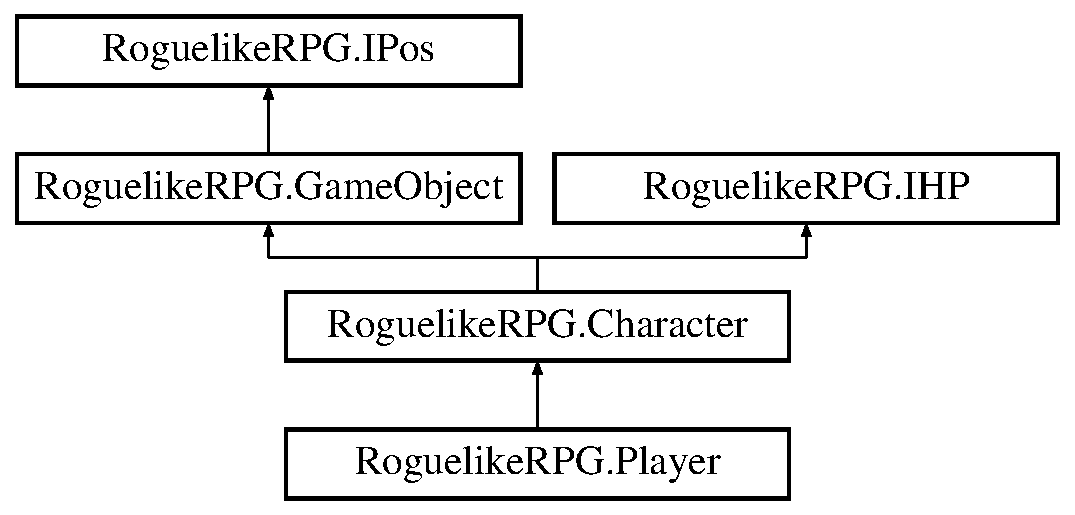
\includegraphics[height=4.000000cm]{class_roguelike_r_p_g_1_1_player}
\end{center}
\end{figure}
\subsection*{Public Member Functions}
\begin{DoxyCompactItemize}
\item 
\mbox{\hyperlink{class_roguelike_r_p_g_1_1_player_a998f3a9a1b1849f460689ec87ce14b72}{Player}} (int X, int Y)
\begin{DoxyCompactList}\small\item\em Initializes the \mbox{\hyperlink{class_roguelike_r_p_g_1_1_player}{Player}} with the given coordinates of X and Y. \end{DoxyCompactList}\item 
void \mbox{\hyperlink{class_roguelike_r_p_g_1_1_player_ac0ed6040b097a55a18e19ee9e604f5de}{Attack}} (\mbox{\hyperlink{class_roguelike_r_p_g_1_1_n_p_c}{N\+PC}} target)
\begin{DoxyCompactList}\small\item\em Attacks the enemy \mbox{\hyperlink{class_roguelike_r_p_g_1_1_n_p_c}{N\+PC}} with current weapon. \end{DoxyCompactList}\item 
void \mbox{\hyperlink{class_roguelike_r_p_g_1_1_player_ae8cdb59fd33dbc6f1b8cc3c17f15908e}{Eat}} (\mbox{\hyperlink{class_roguelike_r_p_g_1_1_food}{Food}} food)
\begin{DoxyCompactList}\small\item\em Consomes Specified \mbox{\hyperlink{class_roguelike_r_p_g_1_1_food}{Food}}. \end{DoxyCompactList}\item 
void \mbox{\hyperlink{class_roguelike_r_p_g_1_1_player_a9851fb6d029e554484fc11bb345b1632}{Pickup\+Item}} (\mbox{\hyperlink{class_roguelike_r_p_g_1_1_item}{Item}} item)
\begin{DoxyCompactList}\small\item\em Picks up specified item. \end{DoxyCompactList}\end{DoxyCompactItemize}
\subsection*{Public Attributes}
\begin{DoxyCompactItemize}
\item 
\mbox{\Hypertarget{class_roguelike_r_p_g_1_1_player_a193007784493dc32f358c748194a9232}\label{class_roguelike_r_p_g_1_1_player_a193007784493dc32f358c748194a9232}} 
List$<$ \mbox{\hyperlink{class_roguelike_r_p_g_1_1_item}{Item}} $>$ {\bfseries Backpack} = new List$<$\mbox{\hyperlink{class_roguelike_r_p_g_1_1_item}{Item}}$>$()
\item 
\mbox{\Hypertarget{class_roguelike_r_p_g_1_1_player_ac63a134363b5f4f73cb1cdd214be81b1}\label{class_roguelike_r_p_g_1_1_player_ac63a134363b5f4f73cb1cdd214be81b1}} 
\mbox{\hyperlink{class_roguelike_r_p_g_1_1_weapon}{Weapon}} {\bfseries Selected\+Weapon}
\end{DoxyCompactItemize}
\subsection*{Additional Inherited Members}


\subsection{Detailed Description}
Class that handles all of the functions in regards to the \mbox{\hyperlink{class_roguelike_r_p_g_1_1_player}{Player}} sub type from \mbox{\hyperlink{class_roguelike_r_p_g_1_1_character}{Character}}. 



\subsection{Constructor \& Destructor Documentation}
\mbox{\Hypertarget{class_roguelike_r_p_g_1_1_player_a998f3a9a1b1849f460689ec87ce14b72}\label{class_roguelike_r_p_g_1_1_player_a998f3a9a1b1849f460689ec87ce14b72}} 
\index{Roguelike\+R\+P\+G\+::\+Player@{Roguelike\+R\+P\+G\+::\+Player}!Player@{Player}}
\index{Player@{Player}!Roguelike\+R\+P\+G\+::\+Player@{Roguelike\+R\+P\+G\+::\+Player}}
\subsubsection{\texorpdfstring{Player()}{Player()}}
{\footnotesize\ttfamily Roguelike\+R\+P\+G.\+Player.\+Player (\begin{DoxyParamCaption}\item[{int}]{X,  }\item[{int}]{Y }\end{DoxyParamCaption})\hspace{0.3cm}{\ttfamily [inline]}}



Initializes the \mbox{\hyperlink{class_roguelike_r_p_g_1_1_player}{Player}} with the given coordinates of X and Y. 


\begin{DoxyParams}{Parameters}
{\em X} & X axis of the player\textquotesingle{}s initial location.\\
\hline
{\em Y} & Y axis of the player\textquotesingle{}s initial location.\\
\hline
\end{DoxyParams}


\subsection{Member Function Documentation}
\mbox{\Hypertarget{class_roguelike_r_p_g_1_1_player_ac0ed6040b097a55a18e19ee9e604f5de}\label{class_roguelike_r_p_g_1_1_player_ac0ed6040b097a55a18e19ee9e604f5de}} 
\index{Roguelike\+R\+P\+G\+::\+Player@{Roguelike\+R\+P\+G\+::\+Player}!Attack@{Attack}}
\index{Attack@{Attack}!Roguelike\+R\+P\+G\+::\+Player@{Roguelike\+R\+P\+G\+::\+Player}}
\subsubsection{\texorpdfstring{Attack()}{Attack()}}
{\footnotesize\ttfamily void Roguelike\+R\+P\+G.\+Player.\+Attack (\begin{DoxyParamCaption}\item[{\mbox{\hyperlink{class_roguelike_r_p_g_1_1_n_p_c}{N\+PC}}}]{target }\end{DoxyParamCaption})\hspace{0.3cm}{\ttfamily [inline]}}



Attacks the enemy \mbox{\hyperlink{class_roguelike_r_p_g_1_1_n_p_c}{N\+PC}} with current weapon. 


\begin{DoxyParams}{Parameters}
{\em target} & Target \mbox{\hyperlink{class_roguelike_r_p_g_1_1_n_p_c}{N\+PC}}\\
\hline
\end{DoxyParams}
\mbox{\Hypertarget{class_roguelike_r_p_g_1_1_player_ae8cdb59fd33dbc6f1b8cc3c17f15908e}\label{class_roguelike_r_p_g_1_1_player_ae8cdb59fd33dbc6f1b8cc3c17f15908e}} 
\index{Roguelike\+R\+P\+G\+::\+Player@{Roguelike\+R\+P\+G\+::\+Player}!Eat@{Eat}}
\index{Eat@{Eat}!Roguelike\+R\+P\+G\+::\+Player@{Roguelike\+R\+P\+G\+::\+Player}}
\subsubsection{\texorpdfstring{Eat()}{Eat()}}
{\footnotesize\ttfamily void Roguelike\+R\+P\+G.\+Player.\+Eat (\begin{DoxyParamCaption}\item[{\mbox{\hyperlink{class_roguelike_r_p_g_1_1_food}{Food}}}]{food }\end{DoxyParamCaption})\hspace{0.3cm}{\ttfamily [inline]}}



Consomes Specified \mbox{\hyperlink{class_roguelike_r_p_g_1_1_food}{Food}}. 


\begin{DoxyParams}{Parameters}
{\em food} & \mbox{\hyperlink{class_roguelike_r_p_g_1_1_food}{Food}} to be eaten\\
\hline
\end{DoxyParams}
\mbox{\Hypertarget{class_roguelike_r_p_g_1_1_player_a9851fb6d029e554484fc11bb345b1632}\label{class_roguelike_r_p_g_1_1_player_a9851fb6d029e554484fc11bb345b1632}} 
\index{Roguelike\+R\+P\+G\+::\+Player@{Roguelike\+R\+P\+G\+::\+Player}!Pickup\+Item@{Pickup\+Item}}
\index{Pickup\+Item@{Pickup\+Item}!Roguelike\+R\+P\+G\+::\+Player@{Roguelike\+R\+P\+G\+::\+Player}}
\subsubsection{\texorpdfstring{Pickup\+Item()}{PickupItem()}}
{\footnotesize\ttfamily void Roguelike\+R\+P\+G.\+Player.\+Pickup\+Item (\begin{DoxyParamCaption}\item[{\mbox{\hyperlink{class_roguelike_r_p_g_1_1_item}{Item}}}]{item }\end{DoxyParamCaption})\hspace{0.3cm}{\ttfamily [inline]}}



Picks up specified item. 


\begin{DoxyParams}{Parameters}
{\em item} & \\
\hline
\end{DoxyParams}


The documentation for this class was generated from the following file\+:\begin{DoxyCompactItemize}
\item 
Player.\+cs\end{DoxyCompactItemize}

\hypertarget{class_roguelike_r_p_g_1_1_program}{}\section{Roguelike\+R\+P\+G.\+Program Class Reference}
\label{class_roguelike_r_p_g_1_1_program}\index{Roguelike\+R\+P\+G.\+Program@{Roguelike\+R\+P\+G.\+Program}}


The documentation for this class was generated from the following file\+:\begin{DoxyCompactItemize}
\item 
Program.\+cs\end{DoxyCompactItemize}

\hypertarget{class_roguelike_r_p_g_1_1_renderer}{}\section{Roguelike\+R\+P\+G.\+Renderer Class Reference}
\label{class_roguelike_r_p_g_1_1_renderer}\index{Roguelike\+R\+P\+G.\+Renderer@{Roguelike\+R\+P\+G.\+Renderer}}


Class that handles of the rendering used.  


\subsection*{Public Member Functions}
\begin{DoxyCompactItemize}
\item 
\mbox{\hyperlink{class_roguelike_r_p_g_1_1_renderer_a398c2192581cc61abc4ad6a0299cab96}{Renderer}} (\mbox{\hyperlink{class_roguelike_r_p_g_1_1_player}{Player}} player, \mbox{\hyperlink{class_roguelike_r_p_g_1_1_grid}{Grid}} grid, \mbox{\hyperlink{class_roguelike_r_p_g_1_1_game_loop}{Game\+Loop}} game\+Loop)
\begin{DoxyCompactList}\small\item\em Initializes the renderer. \end{DoxyCompactList}\item 
void \mbox{\hyperlink{class_roguelike_r_p_g_1_1_renderer_a271d86335afd2b6ef8c2ca673baecb21}{Render\+Start\+Screen}} ()
\begin{DoxyCompactList}\small\item\em Renders the Start Screen with Write\+Line\textquotesingle{}s \end{DoxyCompactList}\item 
void \mbox{\hyperlink{class_roguelike_r_p_g_1_1_renderer_a6d07f00e8ed8c9d2897a24630a0a353c}{Render\+Credits}} ()
\begin{DoxyCompactList}\small\item\em Renders the Credits with Write\+Line\textquotesingle{}s. \end{DoxyCompactList}\item 
void \mbox{\hyperlink{class_roguelike_r_p_g_1_1_renderer_a74f7f40cef19e77afac474d526df9e43}{Render\+UI}} ()
\begin{DoxyCompactList}\small\item\em Renders the UI with Write\+Line\textquotesingle{}s \end{DoxyCompactList}\end{DoxyCompactItemize}


\subsection{Detailed Description}
Class that handles of the rendering used. 



\subsection{Constructor \& Destructor Documentation}
\mbox{\Hypertarget{class_roguelike_r_p_g_1_1_renderer_a398c2192581cc61abc4ad6a0299cab96}\label{class_roguelike_r_p_g_1_1_renderer_a398c2192581cc61abc4ad6a0299cab96}} 
\index{Roguelike\+R\+P\+G\+::\+Renderer@{Roguelike\+R\+P\+G\+::\+Renderer}!Renderer@{Renderer}}
\index{Renderer@{Renderer}!Roguelike\+R\+P\+G\+::\+Renderer@{Roguelike\+R\+P\+G\+::\+Renderer}}
\subsubsection{\texorpdfstring{Renderer()}{Renderer()}}
{\footnotesize\ttfamily Roguelike\+R\+P\+G.\+Renderer.\+Renderer (\begin{DoxyParamCaption}\item[{\mbox{\hyperlink{class_roguelike_r_p_g_1_1_player}{Player}}}]{player,  }\item[{\mbox{\hyperlink{class_roguelike_r_p_g_1_1_grid}{Grid}}}]{grid,  }\item[{\mbox{\hyperlink{class_roguelike_r_p_g_1_1_game_loop}{Game\+Loop}}}]{game\+Loop }\end{DoxyParamCaption})\hspace{0.3cm}{\ttfamily [inline]}}



Initializes the renderer. 


\begin{DoxyParams}{Parameters}
{\em player} & \\
\hline
{\em grid} & \\
\hline
{\em game\+Loop} & \\
\hline
\end{DoxyParams}


\subsection{Member Function Documentation}
\mbox{\Hypertarget{class_roguelike_r_p_g_1_1_renderer_a6d07f00e8ed8c9d2897a24630a0a353c}\label{class_roguelike_r_p_g_1_1_renderer_a6d07f00e8ed8c9d2897a24630a0a353c}} 
\index{Roguelike\+R\+P\+G\+::\+Renderer@{Roguelike\+R\+P\+G\+::\+Renderer}!Render\+Credits@{Render\+Credits}}
\index{Render\+Credits@{Render\+Credits}!Roguelike\+R\+P\+G\+::\+Renderer@{Roguelike\+R\+P\+G\+::\+Renderer}}
\subsubsection{\texorpdfstring{Render\+Credits()}{RenderCredits()}}
{\footnotesize\ttfamily void Roguelike\+R\+P\+G.\+Renderer.\+Render\+Credits (\begin{DoxyParamCaption}{ }\end{DoxyParamCaption})\hspace{0.3cm}{\ttfamily [inline]}}



Renders the Credits with Write\+Line\textquotesingle{}s. 

\mbox{\Hypertarget{class_roguelike_r_p_g_1_1_renderer_a271d86335afd2b6ef8c2ca673baecb21}\label{class_roguelike_r_p_g_1_1_renderer_a271d86335afd2b6ef8c2ca673baecb21}} 
\index{Roguelike\+R\+P\+G\+::\+Renderer@{Roguelike\+R\+P\+G\+::\+Renderer}!Render\+Start\+Screen@{Render\+Start\+Screen}}
\index{Render\+Start\+Screen@{Render\+Start\+Screen}!Roguelike\+R\+P\+G\+::\+Renderer@{Roguelike\+R\+P\+G\+::\+Renderer}}
\subsubsection{\texorpdfstring{Render\+Start\+Screen()}{RenderStartScreen()}}
{\footnotesize\ttfamily void Roguelike\+R\+P\+G.\+Renderer.\+Render\+Start\+Screen (\begin{DoxyParamCaption}{ }\end{DoxyParamCaption})\hspace{0.3cm}{\ttfamily [inline]}}



Renders the Start Screen with Write\+Line\textquotesingle{}s 

\mbox{\Hypertarget{class_roguelike_r_p_g_1_1_renderer_a74f7f40cef19e77afac474d526df9e43}\label{class_roguelike_r_p_g_1_1_renderer_a74f7f40cef19e77afac474d526df9e43}} 
\index{Roguelike\+R\+P\+G\+::\+Renderer@{Roguelike\+R\+P\+G\+::\+Renderer}!Render\+UI@{Render\+UI}}
\index{Render\+UI@{Render\+UI}!Roguelike\+R\+P\+G\+::\+Renderer@{Roguelike\+R\+P\+G\+::\+Renderer}}
\subsubsection{\texorpdfstring{Render\+U\+I()}{RenderUI()}}
{\footnotesize\ttfamily void Roguelike\+R\+P\+G.\+Renderer.\+Render\+UI (\begin{DoxyParamCaption}{ }\end{DoxyParamCaption})\hspace{0.3cm}{\ttfamily [inline]}}



Renders the UI with Write\+Line\textquotesingle{}s 



The documentation for this class was generated from the following file\+:\begin{DoxyCompactItemize}
\item 
Renderer.\+cs\end{DoxyCompactItemize}

\hypertarget{class_roguelike_r_p_g_1_1_tile}{}\section{Roguelike\+R\+P\+G.\+Tile Class Reference}
\label{class_roguelike_r_p_g_1_1_tile}\index{Roguelike\+R\+P\+G.\+Tile@{Roguelike\+R\+P\+G.\+Tile}}


A Class that is used to populate the grid and to also store objects.  


Inheritance diagram for Roguelike\+R\+P\+G.\+Tile\+:\begin{figure}[H]
\begin{center}
\leavevmode
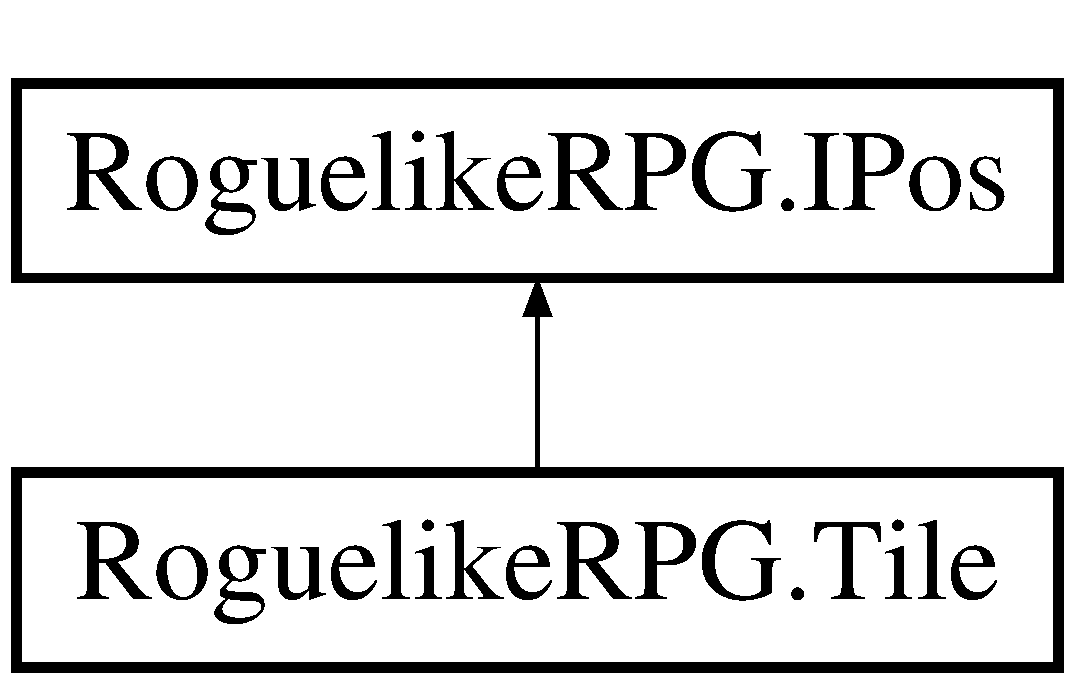
\includegraphics[height=2.000000cm]{class_roguelike_r_p_g_1_1_tile}
\end{center}
\end{figure}
\subsection*{Public Member Functions}
\begin{DoxyCompactItemize}
\item 
void \mbox{\hyperlink{class_roguelike_r_p_g_1_1_tile_a84a16dca9f4ac818eca0eb58f7c5418b}{Remove\+Element}} (\mbox{\hyperlink{class_roguelike_r_p_g_1_1_game_object}{Game\+Object}} obj)
\begin{DoxyCompactList}\small\item\em Used to remove said object in specified tile. \end{DoxyCompactList}\item 
\mbox{\hyperlink{class_roguelike_r_p_g_1_1_tile_ac00f81529ef711a7875d3810749a729d}{Tile}} (int x, int y)
\begin{DoxyCompactList}\small\item\em \mbox{\hyperlink{class_roguelike_r_p_g_1_1_tile}{Tile}} initialization. \end{DoxyCompactList}\item 
void \mbox{\hyperlink{class_roguelike_r_p_g_1_1_tile_a48756f2f22db20e7c765c0d56f5a36f3}{Update\+Pos}} ()
\begin{DoxyCompactList}\small\item\em Updates the position of specified \mbox{\hyperlink{class_roguelike_r_p_g_1_1_game_object}{Game\+Object}} on the tile. \end{DoxyCompactList}\item 
void \mbox{\hyperlink{class_roguelike_r_p_g_1_1_tile_a4540cd9d2fb8989e65778bcffbbe340f}{Add\+Object}} (int ID)
\begin{DoxyCompactList}\small\item\em Adds Objects into tiles \end{DoxyCompactList}\item 
\mbox{\Hypertarget{class_roguelike_r_p_g_1_1_tile_a495e7ee559a4006f4e845ab348b70333}\label{class_roguelike_r_p_g_1_1_tile_a495e7ee559a4006f4e845ab348b70333}} 
override string {\bfseries To\+String} ()
\end{DoxyCompactItemize}
\subsection*{Public Attributes}
\begin{DoxyCompactItemize}
\item 
\mbox{\Hypertarget{class_roguelike_r_p_g_1_1_tile_acaff404969d6ec22a857844a3da768e6}\label{class_roguelike_r_p_g_1_1_tile_acaff404969d6ec22a857844a3da768e6}} 
Stack$<$ \mbox{\hyperlink{class_roguelike_r_p_g_1_1_game_object}{Game\+Object}} $>$ {\bfseries Objects} = new Stack$<$\mbox{\hyperlink{class_roguelike_r_p_g_1_1_game_object}{Game\+Object}}$>$()
\end{DoxyCompactItemize}
\subsection*{Properties}
\begin{DoxyCompactItemize}
\item 
int \mbox{\hyperlink{class_roguelike_r_p_g_1_1_tile_aa70af4c518d3e04eb0488460ebbbb091}{X}}\hspace{0.3cm}{\ttfamily  \mbox{[}get, set\mbox{]}}
\begin{DoxyCompactList}\small\item\em Defines its position in the \mbox{\hyperlink{class_roguelike_r_p_g_1_1_grid}{Grid}} on the X axis. \end{DoxyCompactList}\item 
int \mbox{\hyperlink{class_roguelike_r_p_g_1_1_tile_abc0553a51f38c39df5d62a6595b9552f}{Y}}\hspace{0.3cm}{\ttfamily  \mbox{[}get, set\mbox{]}}
\begin{DoxyCompactList}\small\item\em Defines its position in the \mbox{\hyperlink{class_roguelike_r_p_g_1_1_grid}{Grid}} on the Y axis. \end{DoxyCompactList}\item 
bool \mbox{\hyperlink{class_roguelike_r_p_g_1_1_tile_a1cee19c16fed5cfdd655487f5e79e5c8}{Unknown}}\hspace{0.3cm}{\ttfamily  \mbox{[}get, set\mbox{]}}
\begin{DoxyCompactList}\small\item\em Manages the Fog of war element by holding the information that it has already been found or has yet to be found. \end{DoxyCompactList}\item 
bool \mbox{\hyperlink{class_roguelike_r_p_g_1_1_tile_a67c61a973f25af77d07a12e50b3825f2}{Is\+Exit}}\hspace{0.3cm}{\ttfamily  \mbox{[}get, set\mbox{]}}
\end{DoxyCompactItemize}


\subsection{Detailed Description}
A Class that is used to populate the grid and to also store objects. 



\subsection{Constructor \& Destructor Documentation}
\mbox{\Hypertarget{class_roguelike_r_p_g_1_1_tile_ac00f81529ef711a7875d3810749a729d}\label{class_roguelike_r_p_g_1_1_tile_ac00f81529ef711a7875d3810749a729d}} 
\index{Roguelike\+R\+P\+G\+::\+Tile@{Roguelike\+R\+P\+G\+::\+Tile}!Tile@{Tile}}
\index{Tile@{Tile}!Roguelike\+R\+P\+G\+::\+Tile@{Roguelike\+R\+P\+G\+::\+Tile}}
\subsubsection{\texorpdfstring{Tile()}{Tile()}}
{\footnotesize\ttfamily Roguelike\+R\+P\+G.\+Tile.\+Tile (\begin{DoxyParamCaption}\item[{int}]{x,  }\item[{int}]{y }\end{DoxyParamCaption})\hspace{0.3cm}{\ttfamily [inline]}}



\mbox{\hyperlink{class_roguelike_r_p_g_1_1_tile}{Tile}} initialization. 


\begin{DoxyParams}{Parameters}
{\em x} & \\
\hline
{\em y} & \\
\hline
\end{DoxyParams}


\subsection{Member Function Documentation}
\mbox{\Hypertarget{class_roguelike_r_p_g_1_1_tile_a4540cd9d2fb8989e65778bcffbbe340f}\label{class_roguelike_r_p_g_1_1_tile_a4540cd9d2fb8989e65778bcffbbe340f}} 
\index{Roguelike\+R\+P\+G\+::\+Tile@{Roguelike\+R\+P\+G\+::\+Tile}!Add\+Object@{Add\+Object}}
\index{Add\+Object@{Add\+Object}!Roguelike\+R\+P\+G\+::\+Tile@{Roguelike\+R\+P\+G\+::\+Tile}}
\subsubsection{\texorpdfstring{Add\+Object()}{AddObject()}}
{\footnotesize\ttfamily void Roguelike\+R\+P\+G.\+Tile.\+Add\+Object (\begin{DoxyParamCaption}\item[{int}]{ID }\end{DoxyParamCaption})\hspace{0.3cm}{\ttfamily [inline]}}



Adds Objects into tiles 


\begin{DoxyParams}{Parameters}
{\em ID} & \\
\hline
\end{DoxyParams}
\mbox{\Hypertarget{class_roguelike_r_p_g_1_1_tile_a84a16dca9f4ac818eca0eb58f7c5418b}\label{class_roguelike_r_p_g_1_1_tile_a84a16dca9f4ac818eca0eb58f7c5418b}} 
\index{Roguelike\+R\+P\+G\+::\+Tile@{Roguelike\+R\+P\+G\+::\+Tile}!Remove\+Element@{Remove\+Element}}
\index{Remove\+Element@{Remove\+Element}!Roguelike\+R\+P\+G\+::\+Tile@{Roguelike\+R\+P\+G\+::\+Tile}}
\subsubsection{\texorpdfstring{Remove\+Element()}{RemoveElement()}}
{\footnotesize\ttfamily void Roguelike\+R\+P\+G.\+Tile.\+Remove\+Element (\begin{DoxyParamCaption}\item[{\mbox{\hyperlink{class_roguelike_r_p_g_1_1_game_object}{Game\+Object}}}]{obj }\end{DoxyParamCaption})\hspace{0.3cm}{\ttfamily [inline]}}



Used to remove said object in specified tile. 


\begin{DoxyParams}{Parameters}
{\em obj} & Object to be removed.\\
\hline
\end{DoxyParams}
\mbox{\Hypertarget{class_roguelike_r_p_g_1_1_tile_a48756f2f22db20e7c765c0d56f5a36f3}\label{class_roguelike_r_p_g_1_1_tile_a48756f2f22db20e7c765c0d56f5a36f3}} 
\index{Roguelike\+R\+P\+G\+::\+Tile@{Roguelike\+R\+P\+G\+::\+Tile}!Update\+Pos@{Update\+Pos}}
\index{Update\+Pos@{Update\+Pos}!Roguelike\+R\+P\+G\+::\+Tile@{Roguelike\+R\+P\+G\+::\+Tile}}
\subsubsection{\texorpdfstring{Update\+Pos()}{UpdatePos()}}
{\footnotesize\ttfamily void Roguelike\+R\+P\+G.\+Tile.\+Update\+Pos (\begin{DoxyParamCaption}{ }\end{DoxyParamCaption})\hspace{0.3cm}{\ttfamily [inline]}}



Updates the position of specified \mbox{\hyperlink{class_roguelike_r_p_g_1_1_game_object}{Game\+Object}} on the tile. 



\subsection{Property Documentation}
\mbox{\Hypertarget{class_roguelike_r_p_g_1_1_tile_a67c61a973f25af77d07a12e50b3825f2}\label{class_roguelike_r_p_g_1_1_tile_a67c61a973f25af77d07a12e50b3825f2}} 
\index{Roguelike\+R\+P\+G\+::\+Tile@{Roguelike\+R\+P\+G\+::\+Tile}!Is\+Exit@{Is\+Exit}}
\index{Is\+Exit@{Is\+Exit}!Roguelike\+R\+P\+G\+::\+Tile@{Roguelike\+R\+P\+G\+::\+Tile}}
\subsubsection{\texorpdfstring{Is\+Exit}{IsExit}}
{\footnotesize\ttfamily bool Roguelike\+R\+P\+G.\+Tile.\+Is\+Exit\hspace{0.3cm}{\ttfamily [get]}, {\ttfamily [set]}}





\mbox{\Hypertarget{class_roguelike_r_p_g_1_1_tile_a1cee19c16fed5cfdd655487f5e79e5c8}\label{class_roguelike_r_p_g_1_1_tile_a1cee19c16fed5cfdd655487f5e79e5c8}} 
\index{Roguelike\+R\+P\+G\+::\+Tile@{Roguelike\+R\+P\+G\+::\+Tile}!Unknown@{Unknown}}
\index{Unknown@{Unknown}!Roguelike\+R\+P\+G\+::\+Tile@{Roguelike\+R\+P\+G\+::\+Tile}}
\subsubsection{\texorpdfstring{Unknown}{Unknown}}
{\footnotesize\ttfamily bool Roguelike\+R\+P\+G.\+Tile.\+Unknown\hspace{0.3cm}{\ttfamily [get]}, {\ttfamily [set]}}



Manages the Fog of war element by holding the information that it has already been found or has yet to be found. 

\mbox{\Hypertarget{class_roguelike_r_p_g_1_1_tile_aa70af4c518d3e04eb0488460ebbbb091}\label{class_roguelike_r_p_g_1_1_tile_aa70af4c518d3e04eb0488460ebbbb091}} 
\index{Roguelike\+R\+P\+G\+::\+Tile@{Roguelike\+R\+P\+G\+::\+Tile}!X@{X}}
\index{X@{X}!Roguelike\+R\+P\+G\+::\+Tile@{Roguelike\+R\+P\+G\+::\+Tile}}
\subsubsection{\texorpdfstring{X}{X}}
{\footnotesize\ttfamily int Roguelike\+R\+P\+G.\+Tile.\+X\hspace{0.3cm}{\ttfamily [get]}, {\ttfamily [set]}}



Defines its position in the \mbox{\hyperlink{class_roguelike_r_p_g_1_1_grid}{Grid}} on the X axis. 

\mbox{\Hypertarget{class_roguelike_r_p_g_1_1_tile_abc0553a51f38c39df5d62a6595b9552f}\label{class_roguelike_r_p_g_1_1_tile_abc0553a51f38c39df5d62a6595b9552f}} 
\index{Roguelike\+R\+P\+G\+::\+Tile@{Roguelike\+R\+P\+G\+::\+Tile}!Y@{Y}}
\index{Y@{Y}!Roguelike\+R\+P\+G\+::\+Tile@{Roguelike\+R\+P\+G\+::\+Tile}}
\subsubsection{\texorpdfstring{Y}{Y}}
{\footnotesize\ttfamily int Roguelike\+R\+P\+G.\+Tile.\+Y\hspace{0.3cm}{\ttfamily [get]}, {\ttfamily [set]}}



Defines its position in the \mbox{\hyperlink{class_roguelike_r_p_g_1_1_grid}{Grid}} on the Y axis. 



The documentation for this class was generated from the following file\+:\begin{DoxyCompactItemize}
\item 
Tile.\+cs\end{DoxyCompactItemize}

\hypertarget{class_roguelike_r_p_g_1_1_trap}{}\section{Roguelike\+R\+P\+G.\+Trap Class Reference}
\label{class_roguelike_r_p_g_1_1_trap}\index{Roguelike\+R\+P\+G.\+Trap@{Roguelike\+R\+P\+G.\+Trap}}


Class that handles all of the functions in regards to the \mbox{\hyperlink{class_roguelike_r_p_g_1_1_trap}{Trap}} sub type from \mbox{\hyperlink{class_roguelike_r_p_g_1_1_game_object}{Game\+Object}}.  


Inheritance diagram for Roguelike\+R\+P\+G.\+Trap\+:\begin{figure}[H]
\begin{center}
\leavevmode
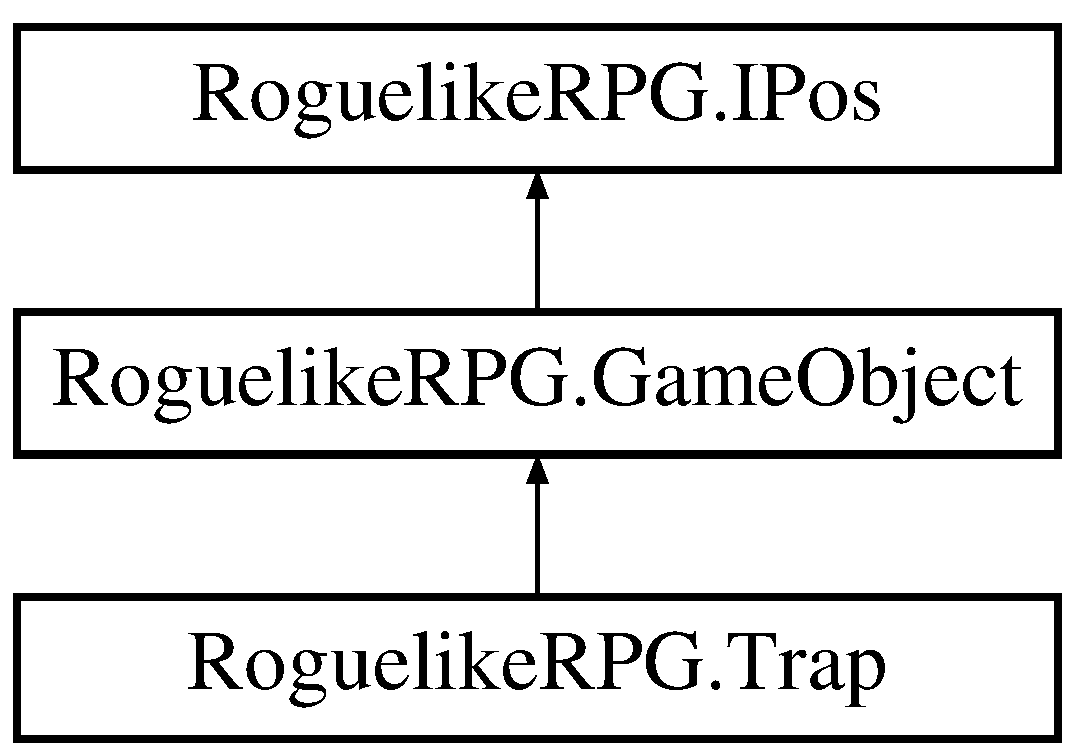
\includegraphics[height=3.000000cm]{class_roguelike_r_p_g_1_1_trap}
\end{center}
\end{figure}
\subsection*{Public Member Functions}
\begin{DoxyCompactItemize}
\item 
\mbox{\hyperlink{class_roguelike_r_p_g_1_1_trap_a75f7e3f09db85a57be63fea667c72ad9}{Trap}} (\mbox{\hyperlink{struct_roguelike_r_p_g_1_1_object_data}{Object\+Data}} obj, int x, int y)
\begin{DoxyCompactList}\small\item\em Handles initialization of the \mbox{\hyperlink{class_roguelike_r_p_g_1_1_trap}{Trap}} object. \end{DoxyCompactList}\item 
void \mbox{\hyperlink{class_roguelike_r_p_g_1_1_trap_a29a26903d96d45aee7a705fdbb191418}{Trap\+Action}} (\mbox{\hyperlink{class_roguelike_r_p_g_1_1_grid}{Grid}} grid)
\begin{DoxyCompactList}\small\item\em Checks if the player is in a trap tile in the grid, checks if said trap is triggered already or not and finally deals damage if it hasnt been triggered already. Causing the Traps state to be Triggered. \end{DoxyCompactList}\end{DoxyCompactItemize}
\subsection*{Properties}
\begin{DoxyCompactItemize}
\item 
bool \mbox{\hyperlink{class_roguelike_r_p_g_1_1_trap_a2be484e07ac0dba84b5f1a8d5235db67}{Triggered}}\hspace{0.3cm}{\ttfamily  \mbox{[}get, set\mbox{]}}
\begin{DoxyCompactList}\small\item\em Handles the managment of the \mbox{\hyperlink{class_roguelike_r_p_g_1_1_trap}{Trap}}\textquotesingle{}s State of being Triggered. \end{DoxyCompactList}\item 
float \mbox{\hyperlink{class_roguelike_r_p_g_1_1_trap_a4a52d250eebe047304262c389b4f82c7}{Max\+Damage}}\hspace{0.3cm}{\ttfamily  \mbox{[}get\mbox{]}}
\begin{DoxyCompactList}\small\item\em Handles the managment of the \mbox{\hyperlink{class_roguelike_r_p_g_1_1_trap}{Trap}}\textquotesingle{}s Max Damage, cannot be changed. \end{DoxyCompactList}\end{DoxyCompactItemize}


\subsection{Detailed Description}
Class that handles all of the functions in regards to the \mbox{\hyperlink{class_roguelike_r_p_g_1_1_trap}{Trap}} sub type from \mbox{\hyperlink{class_roguelike_r_p_g_1_1_game_object}{Game\+Object}}. 



\subsection{Constructor \& Destructor Documentation}
\mbox{\Hypertarget{class_roguelike_r_p_g_1_1_trap_a75f7e3f09db85a57be63fea667c72ad9}\label{class_roguelike_r_p_g_1_1_trap_a75f7e3f09db85a57be63fea667c72ad9}} 
\index{Roguelike\+R\+P\+G\+::\+Trap@{Roguelike\+R\+P\+G\+::\+Trap}!Trap@{Trap}}
\index{Trap@{Trap}!Roguelike\+R\+P\+G\+::\+Trap@{Roguelike\+R\+P\+G\+::\+Trap}}
\subsubsection{\texorpdfstring{Trap()}{Trap()}}
{\footnotesize\ttfamily Roguelike\+R\+P\+G.\+Trap.\+Trap (\begin{DoxyParamCaption}\item[{\mbox{\hyperlink{struct_roguelike_r_p_g_1_1_object_data}{Object\+Data}}}]{obj,  }\item[{int}]{x,  }\item[{int}]{y }\end{DoxyParamCaption})\hspace{0.3cm}{\ttfamily [inline]}}



Handles initialization of the \mbox{\hyperlink{class_roguelike_r_p_g_1_1_trap}{Trap}} object. 


\begin{DoxyParams}{Parameters}
{\em obj} & \\
\hline
{\em x} & \\
\hline
{\em y} & \\
\hline
\end{DoxyParams}


\subsection{Member Function Documentation}
\mbox{\Hypertarget{class_roguelike_r_p_g_1_1_trap_a29a26903d96d45aee7a705fdbb191418}\label{class_roguelike_r_p_g_1_1_trap_a29a26903d96d45aee7a705fdbb191418}} 
\index{Roguelike\+R\+P\+G\+::\+Trap@{Roguelike\+R\+P\+G\+::\+Trap}!Trap\+Action@{Trap\+Action}}
\index{Trap\+Action@{Trap\+Action}!Roguelike\+R\+P\+G\+::\+Trap@{Roguelike\+R\+P\+G\+::\+Trap}}
\subsubsection{\texorpdfstring{Trap\+Action()}{TrapAction()}}
{\footnotesize\ttfamily void Roguelike\+R\+P\+G.\+Trap.\+Trap\+Action (\begin{DoxyParamCaption}\item[{\mbox{\hyperlink{class_roguelike_r_p_g_1_1_grid}{Grid}}}]{grid }\end{DoxyParamCaption})\hspace{0.3cm}{\ttfamily [inline]}}



Checks if the player is in a trap tile in the grid, checks if said trap is triggered already or not and finally deals damage if it hasnt been triggered already. Causing the Traps state to be Triggered. 


\begin{DoxyParams}{Parameters}
{\em grid} & Specified \mbox{\hyperlink{class_roguelike_r_p_g_1_1_grid}{Grid}}\\
\hline
\end{DoxyParams}


\subsection{Property Documentation}
\mbox{\Hypertarget{class_roguelike_r_p_g_1_1_trap_a4a52d250eebe047304262c389b4f82c7}\label{class_roguelike_r_p_g_1_1_trap_a4a52d250eebe047304262c389b4f82c7}} 
\index{Roguelike\+R\+P\+G\+::\+Trap@{Roguelike\+R\+P\+G\+::\+Trap}!Max\+Damage@{Max\+Damage}}
\index{Max\+Damage@{Max\+Damage}!Roguelike\+R\+P\+G\+::\+Trap@{Roguelike\+R\+P\+G\+::\+Trap}}
\subsubsection{\texorpdfstring{Max\+Damage}{MaxDamage}}
{\footnotesize\ttfamily float Roguelike\+R\+P\+G.\+Trap.\+Max\+Damage\hspace{0.3cm}{\ttfamily [get]}}



Handles the managment of the \mbox{\hyperlink{class_roguelike_r_p_g_1_1_trap}{Trap}}\textquotesingle{}s Max Damage, cannot be changed. 

\mbox{\Hypertarget{class_roguelike_r_p_g_1_1_trap_a2be484e07ac0dba84b5f1a8d5235db67}\label{class_roguelike_r_p_g_1_1_trap_a2be484e07ac0dba84b5f1a8d5235db67}} 
\index{Roguelike\+R\+P\+G\+::\+Trap@{Roguelike\+R\+P\+G\+::\+Trap}!Triggered@{Triggered}}
\index{Triggered@{Triggered}!Roguelike\+R\+P\+G\+::\+Trap@{Roguelike\+R\+P\+G\+::\+Trap}}
\subsubsection{\texorpdfstring{Triggered}{Triggered}}
{\footnotesize\ttfamily bool Roguelike\+R\+P\+G.\+Trap.\+Triggered\hspace{0.3cm}{\ttfamily [get]}, {\ttfamily [set]}}



Handles the managment of the \mbox{\hyperlink{class_roguelike_r_p_g_1_1_trap}{Trap}}\textquotesingle{}s State of being Triggered. 



The documentation for this class was generated from the following file\+:\begin{DoxyCompactItemize}
\item 
Trap.\+cs\end{DoxyCompactItemize}

\hypertarget{class_roguelike_r_p_g_1_1_weapon}{}\section{Roguelike\+R\+P\+G.\+Weapon Class Reference}
\label{class_roguelike_r_p_g_1_1_weapon}\index{Roguelike\+R\+P\+G.\+Weapon@{Roguelike\+R\+P\+G.\+Weapon}}


Class that handles all of the functions in regards to the \mbox{\hyperlink{class_roguelike_r_p_g_1_1_weapon}{Weapon}} sub type from items.  


Inheritance diagram for Roguelike\+R\+P\+G.\+Weapon\+:\begin{figure}[H]
\begin{center}
\leavevmode
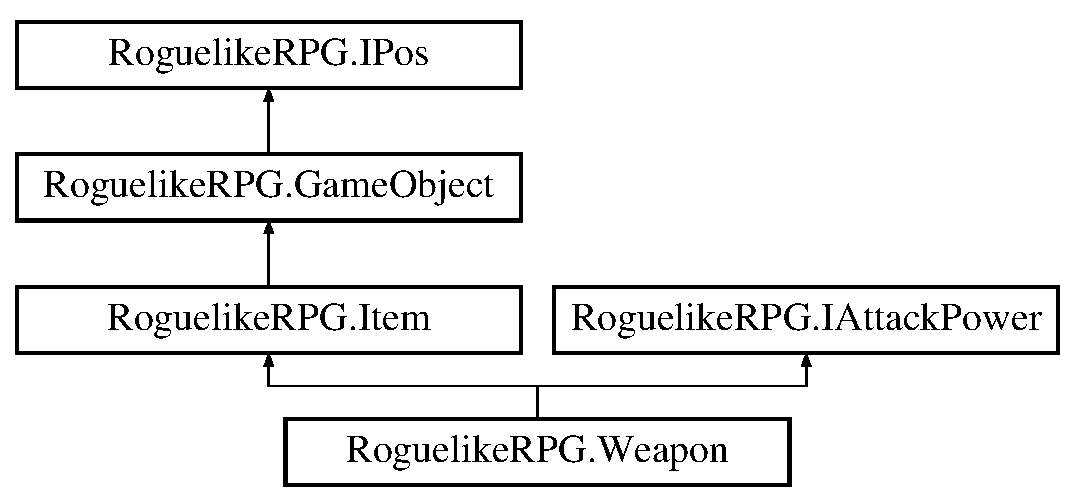
\includegraphics[height=4.000000cm]{class_roguelike_r_p_g_1_1_weapon}
\end{center}
\end{figure}
\subsection*{Public Member Functions}
\begin{DoxyCompactItemize}
\item 
\mbox{\hyperlink{class_roguelike_r_p_g_1_1_weapon_a150f41f8b59b68c93eba9b01efa812b9}{Weapon}} (\mbox{\hyperlink{struct_roguelike_r_p_g_1_1_object_data}{Object\+Data}} obj, int x, int y)
\begin{DoxyCompactList}\small\item\em Handles initialization of the \mbox{\hyperlink{class_roguelike_r_p_g_1_1_weapon}{Weapon}} object. \end{DoxyCompactList}\item 
void \mbox{\hyperlink{class_roguelike_r_p_g_1_1_weapon_abc7ba430a40dc00c52d2ae10a1005eeb}{Use}} (\mbox{\hyperlink{class_roguelike_r_p_g_1_1_n_p_c}{N\+PC}} npc)
\begin{DoxyCompactList}\small\item\em Damages said \mbox{\hyperlink{class_roguelike_r_p_g_1_1_n_p_c}{N\+PC}} with the weapon\textquotesingle{}s Attack Power \end{DoxyCompactList}\item 
void \mbox{\hyperlink{class_roguelike_r_p_g_1_1_weapon_a08c34d6e41739612a4c69fd019fce3d7}{Equip}} (\mbox{\hyperlink{class_roguelike_r_p_g_1_1_player}{Player}} player)
\begin{DoxyCompactList}\small\item\em The \mbox{\hyperlink{class_roguelike_r_p_g_1_1_player}{Player}} equips the selected \mbox{\hyperlink{class_roguelike_r_p_g_1_1_weapon}{Weapon}}. Removing it from his Backpack. \end{DoxyCompactList}\item 
void \mbox{\hyperlink{class_roguelike_r_p_g_1_1_weapon_a583cc9a8265e81bc38d69851bdd6d36a}{Pick\+Up}} (\mbox{\hyperlink{class_roguelike_r_p_g_1_1_player}{Player}} player, \mbox{\hyperlink{class_roguelike_r_p_g_1_1_grid}{Grid}} grid)
\begin{DoxyCompactList}\small\item\em Adds the \mbox{\hyperlink{class_roguelike_r_p_g_1_1_weapon}{Weapon}} to the Backpack of the player, on the \mbox{\hyperlink{class_roguelike_r_p_g_1_1_grid}{Grid}}. Removing it from the \mbox{\hyperlink{class_roguelike_r_p_g_1_1_grid}{Grid}} after. \end{DoxyCompactList}\end{DoxyCompactItemize}
\subsection*{Properties}
\begin{DoxyCompactItemize}
\item 
float \mbox{\hyperlink{class_roguelike_r_p_g_1_1_weapon_a68ffbf4b9ebe1e99d879c18021dba80b}{Attack\+Power}}\hspace{0.3cm}{\ttfamily  \mbox{[}get, set\mbox{]}}
\begin{DoxyCompactList}\small\item\em Handles the managment of the weapon\textquotesingle{}s Attack Power. \end{DoxyCompactList}\end{DoxyCompactItemize}


\subsection{Detailed Description}
Class that handles all of the functions in regards to the \mbox{\hyperlink{class_roguelike_r_p_g_1_1_weapon}{Weapon}} sub type from items. 



\subsection{Constructor \& Destructor Documentation}
\mbox{\Hypertarget{class_roguelike_r_p_g_1_1_weapon_a150f41f8b59b68c93eba9b01efa812b9}\label{class_roguelike_r_p_g_1_1_weapon_a150f41f8b59b68c93eba9b01efa812b9}} 
\index{Roguelike\+R\+P\+G\+::\+Weapon@{Roguelike\+R\+P\+G\+::\+Weapon}!Weapon@{Weapon}}
\index{Weapon@{Weapon}!Roguelike\+R\+P\+G\+::\+Weapon@{Roguelike\+R\+P\+G\+::\+Weapon}}
\subsubsection{\texorpdfstring{Weapon()}{Weapon()}}
{\footnotesize\ttfamily Roguelike\+R\+P\+G.\+Weapon.\+Weapon (\begin{DoxyParamCaption}\item[{\mbox{\hyperlink{struct_roguelike_r_p_g_1_1_object_data}{Object\+Data}}}]{obj,  }\item[{int}]{x,  }\item[{int}]{y }\end{DoxyParamCaption})\hspace{0.3cm}{\ttfamily [inline]}}



Handles initialization of the \mbox{\hyperlink{class_roguelike_r_p_g_1_1_weapon}{Weapon}} object. 


\begin{DoxyParams}{Parameters}
{\em obj} & Struct that holds all of the information regarding the weapon we are initializing\\
\hline
{\em x} & X cordinate\\
\hline
{\em y} & Y cordinate\\
\hline
\end{DoxyParams}


\subsection{Member Function Documentation}
\mbox{\Hypertarget{class_roguelike_r_p_g_1_1_weapon_a08c34d6e41739612a4c69fd019fce3d7}\label{class_roguelike_r_p_g_1_1_weapon_a08c34d6e41739612a4c69fd019fce3d7}} 
\index{Roguelike\+R\+P\+G\+::\+Weapon@{Roguelike\+R\+P\+G\+::\+Weapon}!Equip@{Equip}}
\index{Equip@{Equip}!Roguelike\+R\+P\+G\+::\+Weapon@{Roguelike\+R\+P\+G\+::\+Weapon}}
\subsubsection{\texorpdfstring{Equip()}{Equip()}}
{\footnotesize\ttfamily void Roguelike\+R\+P\+G.\+Weapon.\+Equip (\begin{DoxyParamCaption}\item[{\mbox{\hyperlink{class_roguelike_r_p_g_1_1_player}{Player}}}]{player }\end{DoxyParamCaption})\hspace{0.3cm}{\ttfamily [inline]}}



The \mbox{\hyperlink{class_roguelike_r_p_g_1_1_player}{Player}} equips the selected \mbox{\hyperlink{class_roguelike_r_p_g_1_1_weapon}{Weapon}}. Removing it from his Backpack. 


\begin{DoxyParams}{Parameters}
{\em player} & Specified \mbox{\hyperlink{class_roguelike_r_p_g_1_1_player}{Player}}\\
\hline
\end{DoxyParams}
\mbox{\Hypertarget{class_roguelike_r_p_g_1_1_weapon_a583cc9a8265e81bc38d69851bdd6d36a}\label{class_roguelike_r_p_g_1_1_weapon_a583cc9a8265e81bc38d69851bdd6d36a}} 
\index{Roguelike\+R\+P\+G\+::\+Weapon@{Roguelike\+R\+P\+G\+::\+Weapon}!Pick\+Up@{Pick\+Up}}
\index{Pick\+Up@{Pick\+Up}!Roguelike\+R\+P\+G\+::\+Weapon@{Roguelike\+R\+P\+G\+::\+Weapon}}
\subsubsection{\texorpdfstring{Pick\+Up()}{PickUp()}}
{\footnotesize\ttfamily void Roguelike\+R\+P\+G.\+Weapon.\+Pick\+Up (\begin{DoxyParamCaption}\item[{\mbox{\hyperlink{class_roguelike_r_p_g_1_1_player}{Player}}}]{player,  }\item[{\mbox{\hyperlink{class_roguelike_r_p_g_1_1_grid}{Grid}}}]{grid }\end{DoxyParamCaption})\hspace{0.3cm}{\ttfamily [inline]}}



Adds the \mbox{\hyperlink{class_roguelike_r_p_g_1_1_weapon}{Weapon}} to the Backpack of the player, on the \mbox{\hyperlink{class_roguelike_r_p_g_1_1_grid}{Grid}}. Removing it from the \mbox{\hyperlink{class_roguelike_r_p_g_1_1_grid}{Grid}} after. 


\begin{DoxyParams}{Parameters}
{\em player} & Specified \mbox{\hyperlink{class_roguelike_r_p_g_1_1_player}{Player}}\\
\hline
{\em grid} & Specified \mbox{\hyperlink{class_roguelike_r_p_g_1_1_grid}{Grid}}\\
\hline
\end{DoxyParams}
\mbox{\Hypertarget{class_roguelike_r_p_g_1_1_weapon_abc7ba430a40dc00c52d2ae10a1005eeb}\label{class_roguelike_r_p_g_1_1_weapon_abc7ba430a40dc00c52d2ae10a1005eeb}} 
\index{Roguelike\+R\+P\+G\+::\+Weapon@{Roguelike\+R\+P\+G\+::\+Weapon}!Use@{Use}}
\index{Use@{Use}!Roguelike\+R\+P\+G\+::\+Weapon@{Roguelike\+R\+P\+G\+::\+Weapon}}
\subsubsection{\texorpdfstring{Use()}{Use()}}
{\footnotesize\ttfamily void Roguelike\+R\+P\+G.\+Weapon.\+Use (\begin{DoxyParamCaption}\item[{\mbox{\hyperlink{class_roguelike_r_p_g_1_1_n_p_c}{N\+PC}}}]{npc }\end{DoxyParamCaption})\hspace{0.3cm}{\ttfamily [inline]}}



Damages said \mbox{\hyperlink{class_roguelike_r_p_g_1_1_n_p_c}{N\+PC}} with the weapon\textquotesingle{}s Attack Power 


\begin{DoxyParams}{Parameters}
{\em npc} & Targeted Enemy\\
\hline
\end{DoxyParams}


\subsection{Property Documentation}
\mbox{\Hypertarget{class_roguelike_r_p_g_1_1_weapon_a68ffbf4b9ebe1e99d879c18021dba80b}\label{class_roguelike_r_p_g_1_1_weapon_a68ffbf4b9ebe1e99d879c18021dba80b}} 
\index{Roguelike\+R\+P\+G\+::\+Weapon@{Roguelike\+R\+P\+G\+::\+Weapon}!Attack\+Power@{Attack\+Power}}
\index{Attack\+Power@{Attack\+Power}!Roguelike\+R\+P\+G\+::\+Weapon@{Roguelike\+R\+P\+G\+::\+Weapon}}
\subsubsection{\texorpdfstring{Attack\+Power}{AttackPower}}
{\footnotesize\ttfamily float Roguelike\+R\+P\+G.\+Weapon.\+Attack\+Power\hspace{0.3cm}{\ttfamily [get]}, {\ttfamily [set]}}



Handles the managment of the weapon\textquotesingle{}s Attack Power. 



The documentation for this class was generated from the following file\+:\begin{DoxyCompactItemize}
\item 
Weapon.\+cs\end{DoxyCompactItemize}

%--- End generated contents ---

% Index
\backmatter
\newpage
\phantomsection
\clearemptydoublepage
\addcontentsline{toc}{chapter}{Index}
\printindex

\end{document}
